\documentclass[UTF8,a4paper,10pt]{article}

\usepackage[UTF8]{ctex}
\usepackage[margin=1in]{geometry}
\usepackage{amsmath,amsfonts,bm}
\providecommand{\abs}[1]{\left\lvert#1\right\rvert}
\usepackage{multirow}
\usepackage{graphicx}
\usepackage{subfigure}

\title{从铷蒸汽的饱和吸收光谱中提取有效信息}
\author{陈稼霖\and 蔡吉量\and 金鑫\and 李玮煜\and 薛加民\and 游胤涛}

\begin{document}

\maketitle

\section{摘要}
    气体的吸收光谱中包含着物质组成、能级寿命等重要的信息,是人们研究物质的重要工具. 光谱的增宽是一把双刃剑,一方面,增宽造成了信号峰的重叠,掩盖了光谱中更加精细的结构,另一方面,增宽又为人们提供了气体温度、能级寿命等有效信息. 因此,消除增宽对于光谱测量的不利影响,尽可能地从光谱中提取有用的信息,对物质研究具有重要的意义. 我们利用饱和吸收法测量了铷蒸汽在不同磁场强度下的超精细结构,为了从所得光谱中提取有关铷的有效信息,我们进行了各种尝试:利用峰面积计算了铷蒸汽中两种同位素的比例,由多普勒增宽中估算了铷蒸汽的温度,从饱和吸收烧孔间距中验证了铷原子的超精细结构能级之差,并看到了超精细结构在磁场下演化的过程.

\section{原理介绍}

\subsection{铷原子光谱}

\subsubsection{铷原子光谱的超精细结构}

铷(Rb)是第$37$号元素,核外电子排布为[Kr]5s$^1$. 由于仅有一个$5s$轨道的价电子,基态铷原子的轨道量子数$L=0$,电子总角动量量子数即其自旋量子数$J=S=1/2$,原子态为$5^2S_{1/2}$. 第一激发态铷原子的总轨道量子数$L=1$,自旋量子数$S=1/2$,从而电子总角动量量子数可取$J=1/2$和$3/2$,因此第一激发态有两个原子态:$^2$P$_{1/2}$和$^2$P$_{3/2}$. 本实验测量的是铷原子从$^2$P$_{3/2}$态跃迁至$^2$S$_{1/2}$态对应的谱线. 天然的铷元素包含两种同位素:$^{85}$Rb和$^{87}$Rb,核自旋量子数分别为$I=5/2$和$I=3/2$,这两种同位素在自然界中的丰度分别为$72.17\%$和$27.83\%$. $^{85}$Rb的原子总角动量量子数在$^2$S$_{1/2}$态和$^2$P$_{3/2}$态可分别取$F=2,3$和$F=1,2,3,4$;$^{87}$Rb的原子总角动量量子数在$^2$S$_{1/2}$和$^2$P$_{3/2}$态可分别取$F=1,2$和$F=0,1,2,3$. 两种同位素的各量子数总结如\ref{quantum-number}所示.

\begin{table}[h]
    \centering
    \caption{两种铷同位素的部分状态对应的各量子数}
    \label{quantum-number}
    \begin{tabular}{|c|c|c|c|c|c|c|c|}
    \hline
     & 原子态符号 & $S$ & $L$ & $J$ & 同位素 & $I$ & $F$ \\ \hline
    \multirow{2}{*}{基态} & \multirow{2}{*}{$5^2$S$_{1/2}$} & \multirow{6}{*}{$1/2$} & \multirow{2}{*}{$0$} & \multirow{2}{*}{$1/2$} & $^{85}$Rb & $5/2$ & $2,3$ \\ \cline{6-8} 
     &  &  &  &  & $^{87}$Rb & $3/2$ & $1,2$ \\ \cline{1-2} \cline{4-8} 
    \multirow{4}{*}{第一激发态} & \multirow{2}{*}{$5^2$P$_{1/2}$} &  & \multirow{4}{*}{$1$} & \multirow{2}{*}{$1/2$} & $^{85}$Rb & $5/2$ & $2,3$ \\ \cline{6-8} 
     &  &  &  &  & $^{87}$Rb & $3/2$ & $1,2$ \\ \cline{2-2} \cline{5-8} 
     & \multirow{2}{*}{$5^2$P$_{3/2}$} &  &  & \multirow{2}{*}{$3/2$} & $^{85}$Rb & $5/2$ & $1,2,3,4$ \\ \cline{6-8} 
     &  &  &  &  & $^{87}$Rb & $3/2$ & $0,1,2,3$ \\ \hline
    \end{tabular}
\end{table}

原子核存在磁矩,而核外电子运动在原子核处产生磁场,因此存在所谓的磁偶级超精细相互作用,其引起的能级位移为
\begin{align}
    \Delta E=\frac{a_J}{2}[F(F+1)-J(J+1)-I(I+1)],
\end{align}
其中$a_J$是一个与原子状态有关的常数. 铷原子的超精细结构能级如图\ref{energy-state}所示. 图中所标$^2$P$_{3/2}$态的超精细结构能级分裂的比例接近上式但略微存在偏差,偏差的来源是电四极超精细相互作用:原子核内的电荷分布存在电四极矩,铷原子的基态为$S$态,电子波函数球对称分布,在原子核处的电场梯度为零,故不存在电四极相互作用,而对于激发态$^2$P$_{3/2}$,核外电子在原子核处的电场存在梯度,故存在电四极矩相互作用. 电四极超精细相互作用造成的能量分裂小于磁偶级超精细相互作用,可视其为在电偶极相互作用能级分裂上一个的小修正.

\begin{figure}[ht]
    \centering
    \subfigure[$^{85}$Rb]{
    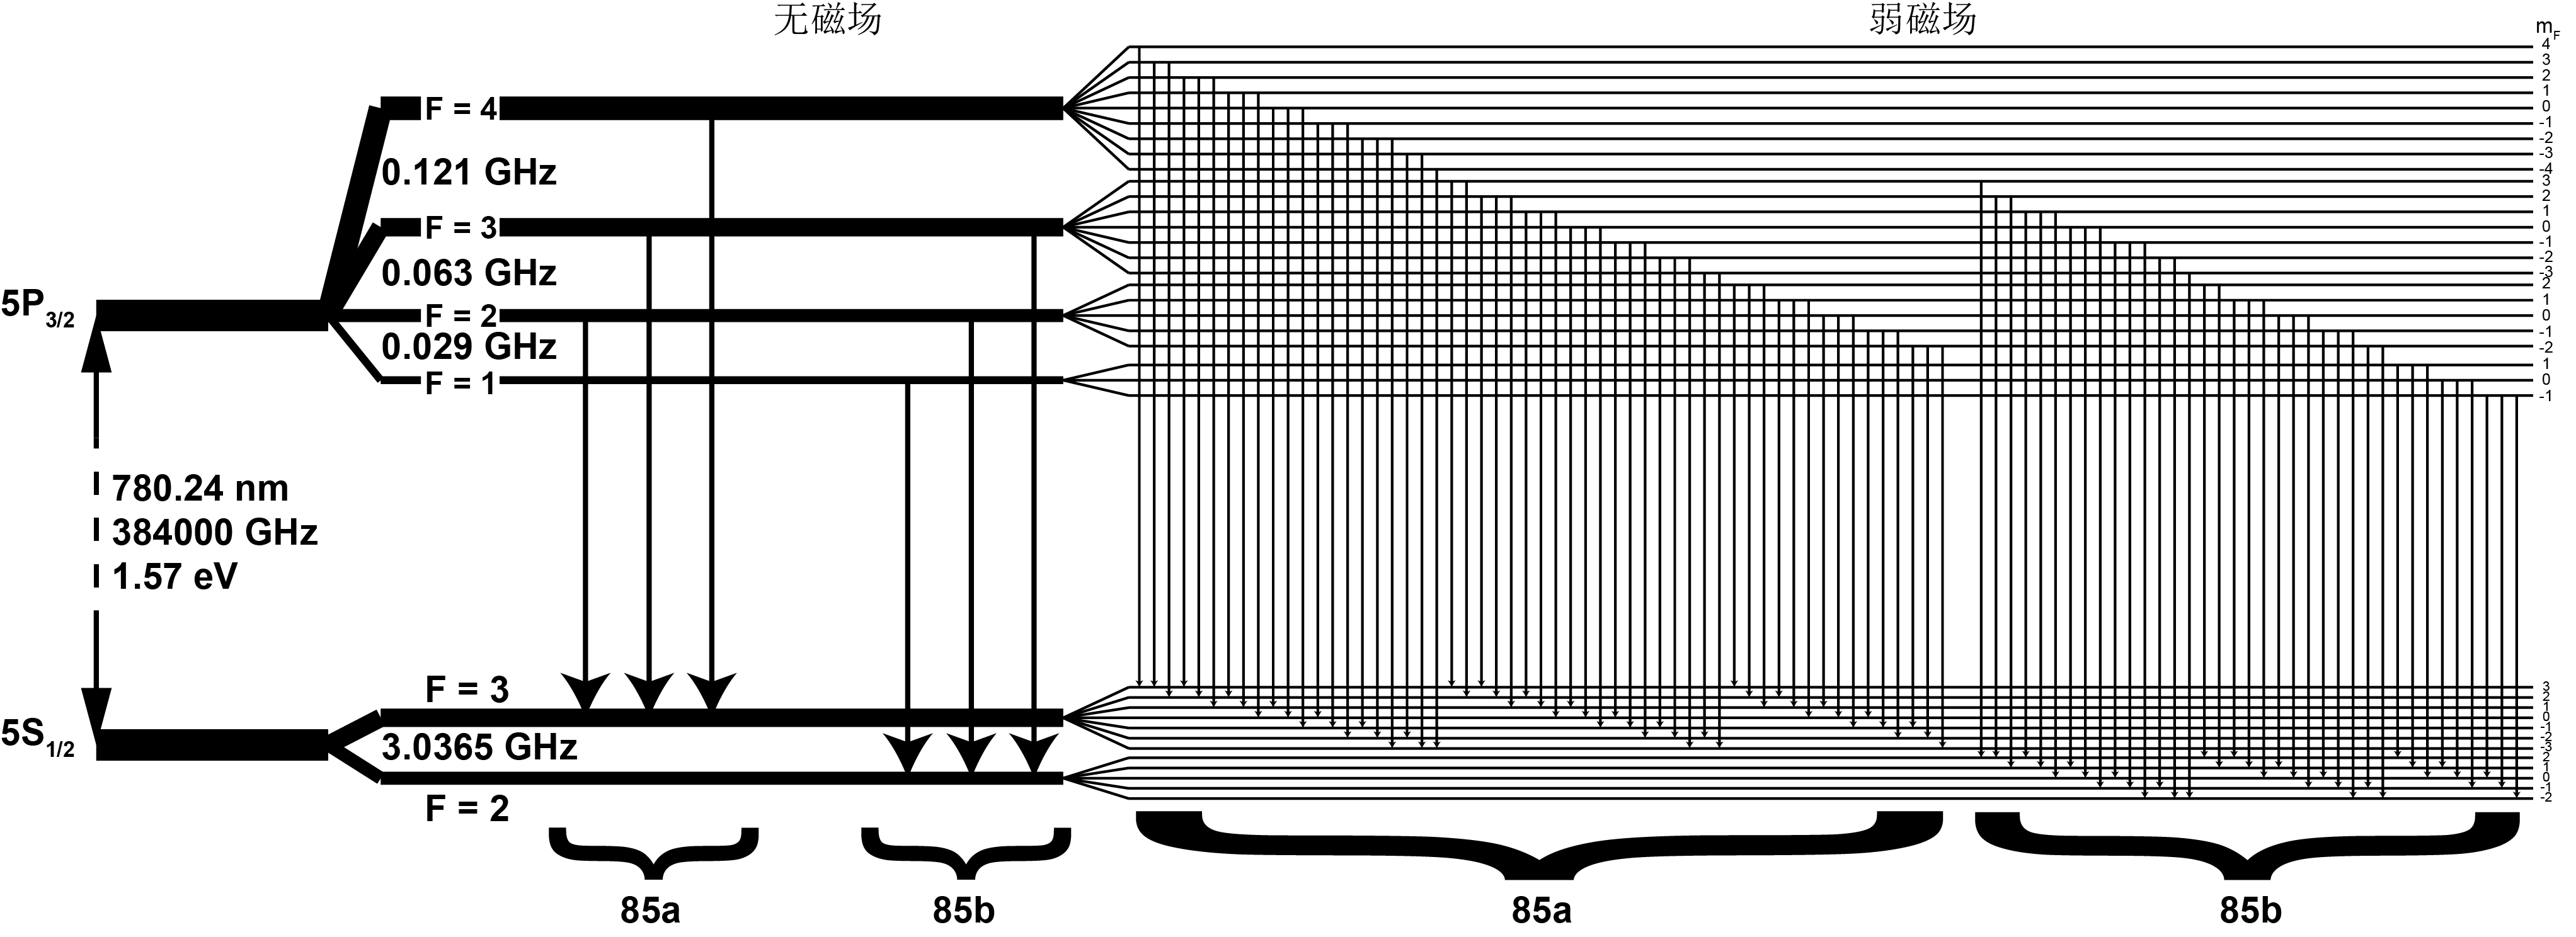
\includegraphics[width=0.8\textwidth]{EnergyState-85.png}}
    \subfigure[$^{87}$Rb]{
    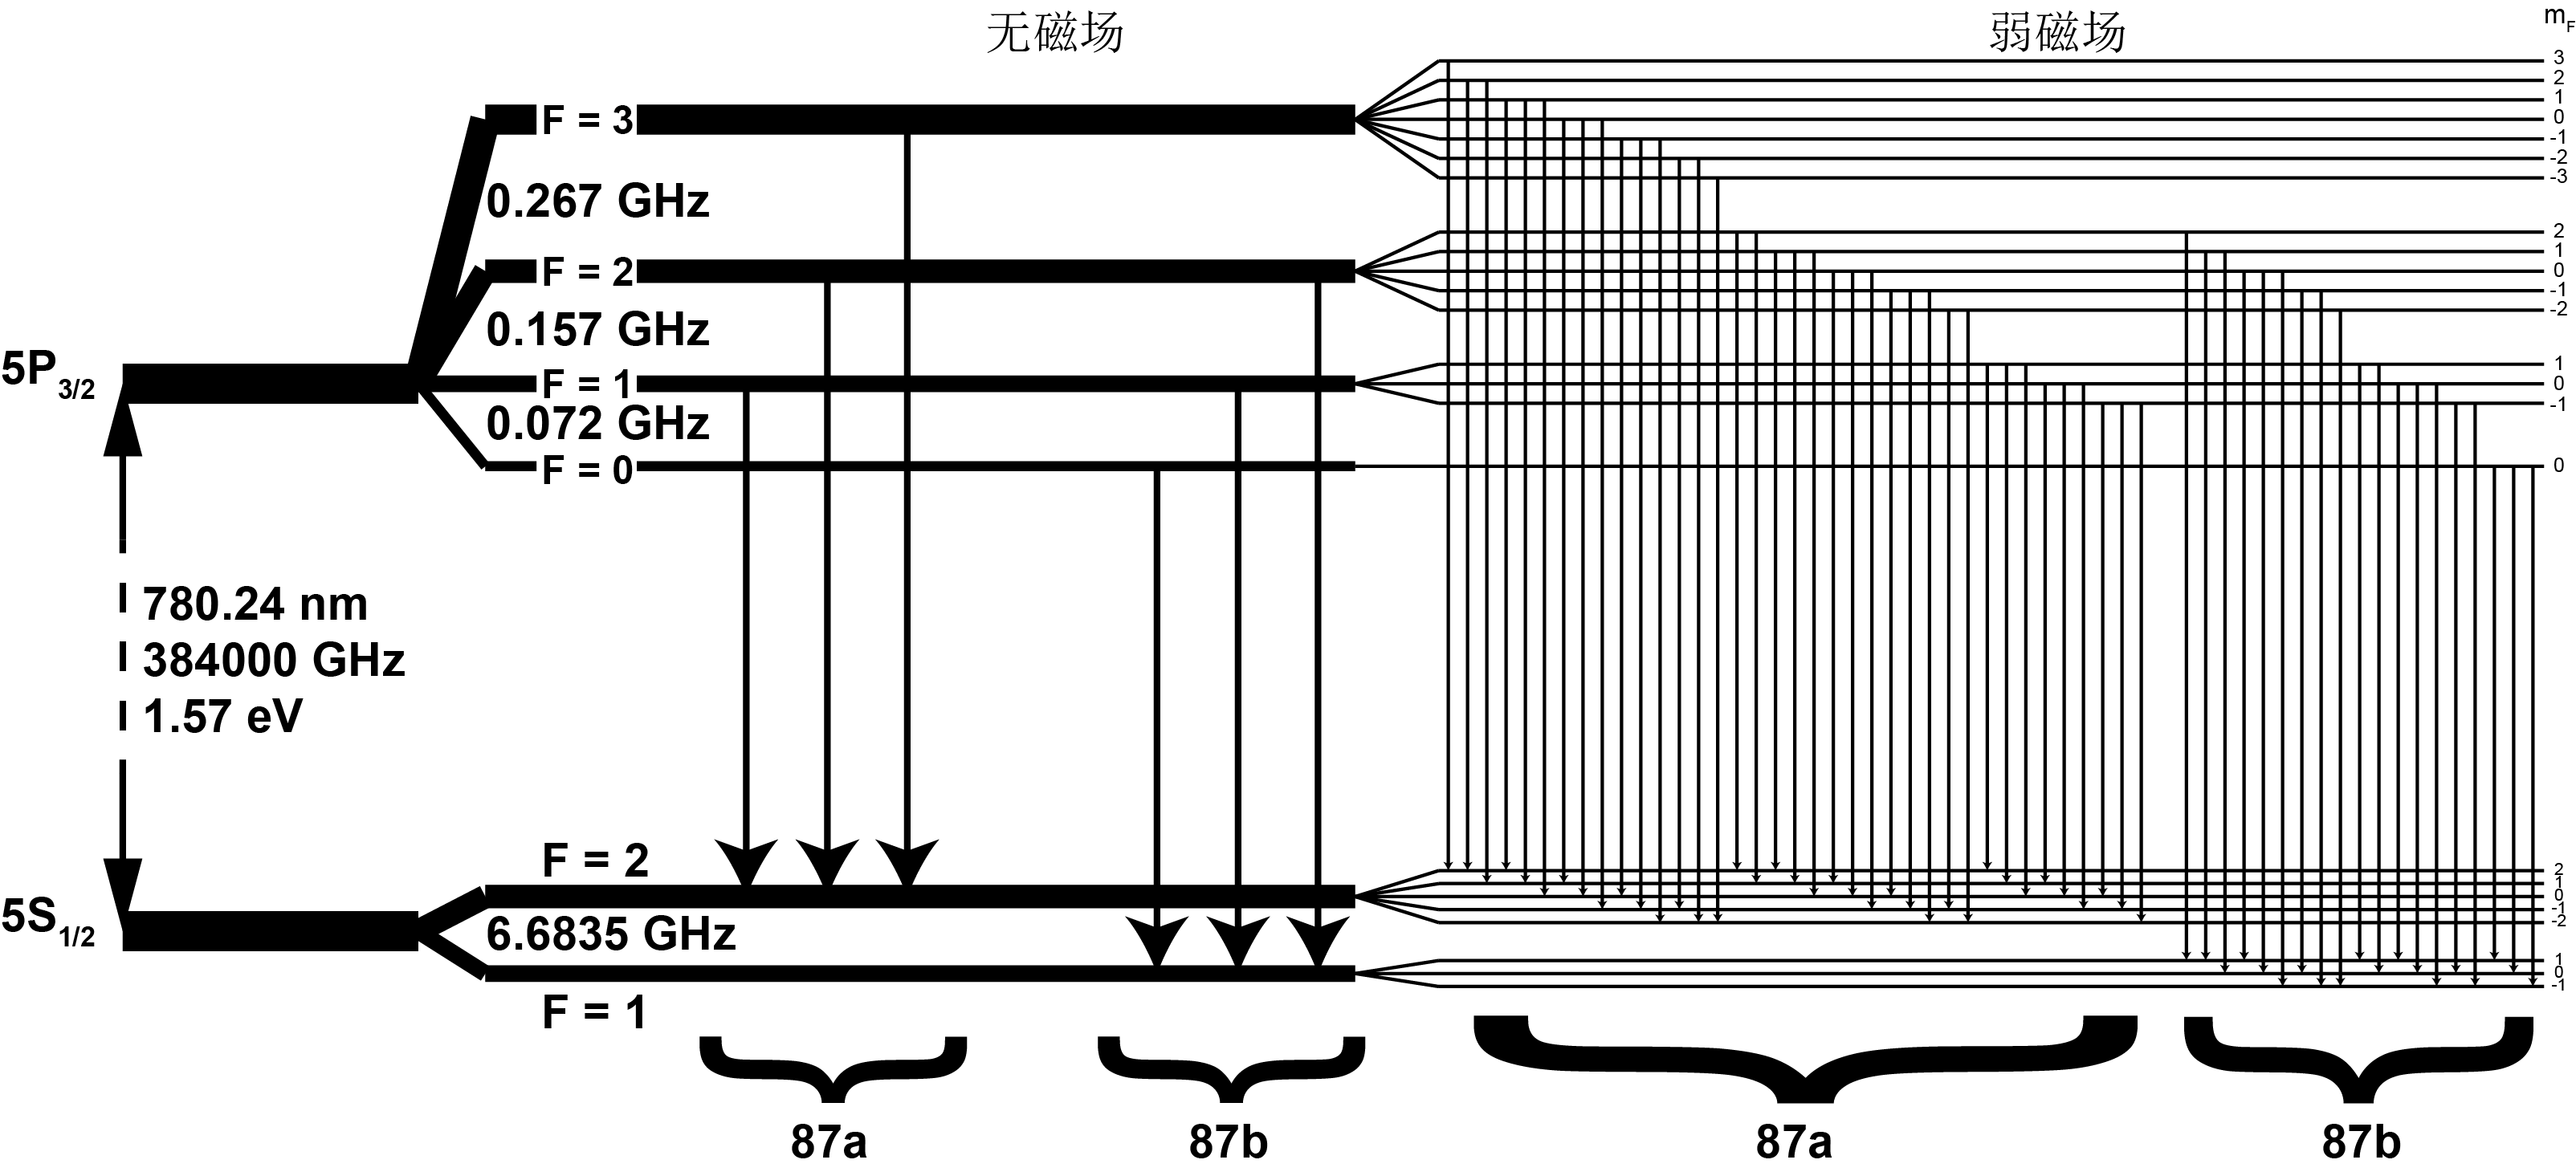
\includegraphics[width=0.8\textwidth]{EnergyState-87.png}}
    \caption{在无磁场和弱磁场下$^{85}$Rb和$^{87}$Rb的部分能级与允许的跃迁.}
    \label{energy-state}
\end{figure}

无磁场下,根据跃迁的选择定则,
\begin{align}
    \Delta F=0,\pm 1,
\end{align}
从$5P_{3/2}$态到$5P_{1/2}$态存在如图\ref{energy-state}所示的跃迁,其中$^{85}$Rb的终态$F=2$的跃迁对应的一系列谱线标号为$85$a,终态$F=3$的跃迁对应的一系列谱线标号为$^{85}$b,$^{87}$Rb的终态$F=1$的跃迁对应的一系列谱线标号为$87$a,终态$F=2$的跃迁对应的一系列谱线标号为$87$b. 每种标号的谱线系实际上各包含三条谱线,但在无饱和吸收的情况下,同一个谱线系中的三条谱线因展宽而相互重叠,在光谱上只表现为一个峰,如图\ref{theoretical-absorption}所示.

\begin{figure}[h]
    \centering
    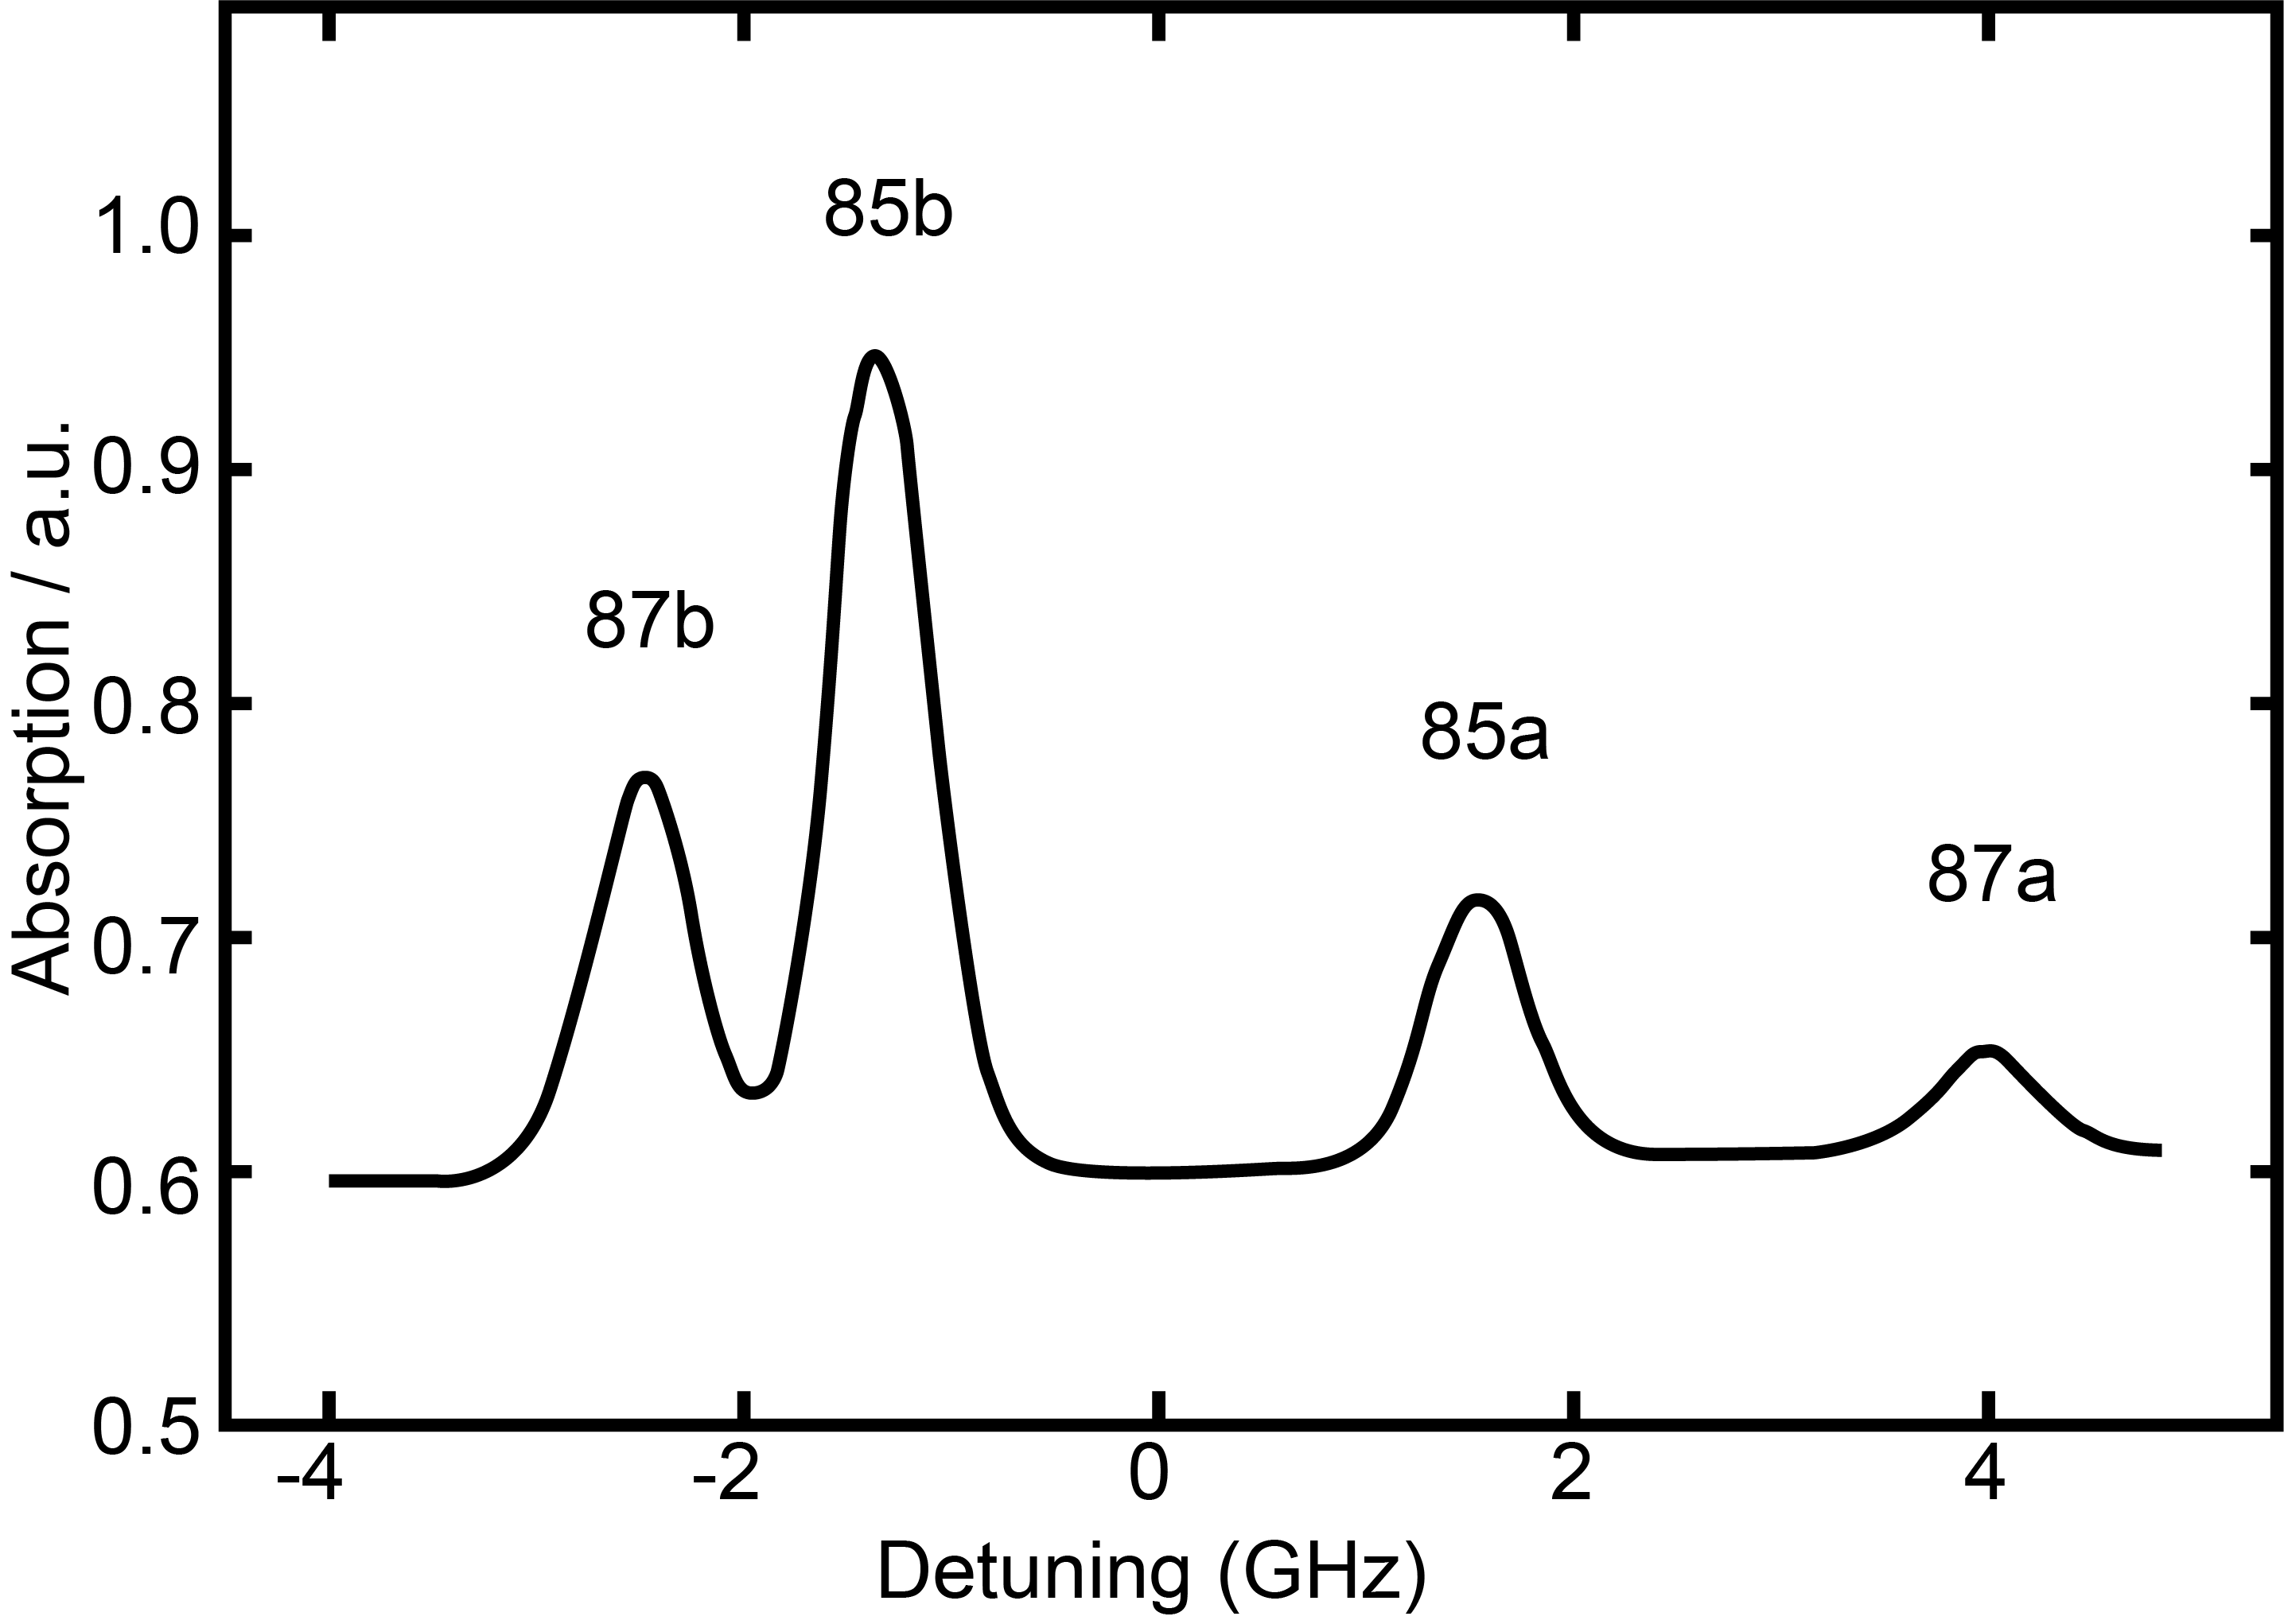
\includegraphics[width=.4\textwidth]{TheoreticalAbsorption.png}
    \caption{Rb蒸汽吸收谱的理论线型.}
    \label{theoretical-absorption}
\end{figure}

\subsubsection{铷原子光谱的超精细结构在磁场下的分裂}

在弱磁场$\bm{B}$下,电子的总自旋角$\bm{J}$仍然先和核自旋$\bm{I}$耦合为原子总自旋$\bm{F}$,$\bm{F}$绕着磁场方向进动,如图\ref{weak-field}所示. $F$在磁场方向的不同投影$m_F$导致了能级分裂:
\begin{align}
    \Delta E=g_Fm_F\mu_BB,
\end{align}
其中$g_F$为原子总自旋的朗德$g$因子,$m_F$可取$-F,-F+1,\cdots,F-1,F$,即原子总自旋量子数为$F$的能级分裂成$2F+1$个能级,如图\ref{energy-state}所示. 这些能级之间的跃迁遵从选择定则,
\begin{gather}
    \Delta F=0,\pm 1,\\
    \Delta m_F=0,\pm 1.
\end{gather}

\begin{figure}[ht]
    \centering
    \subfigure[弱磁场下,$\bm{J}$先与$\bm{I}$耦合为$\bm{F}$,$\bm{F}$绕着磁场方向进动.]{
    \label{weak-field}
    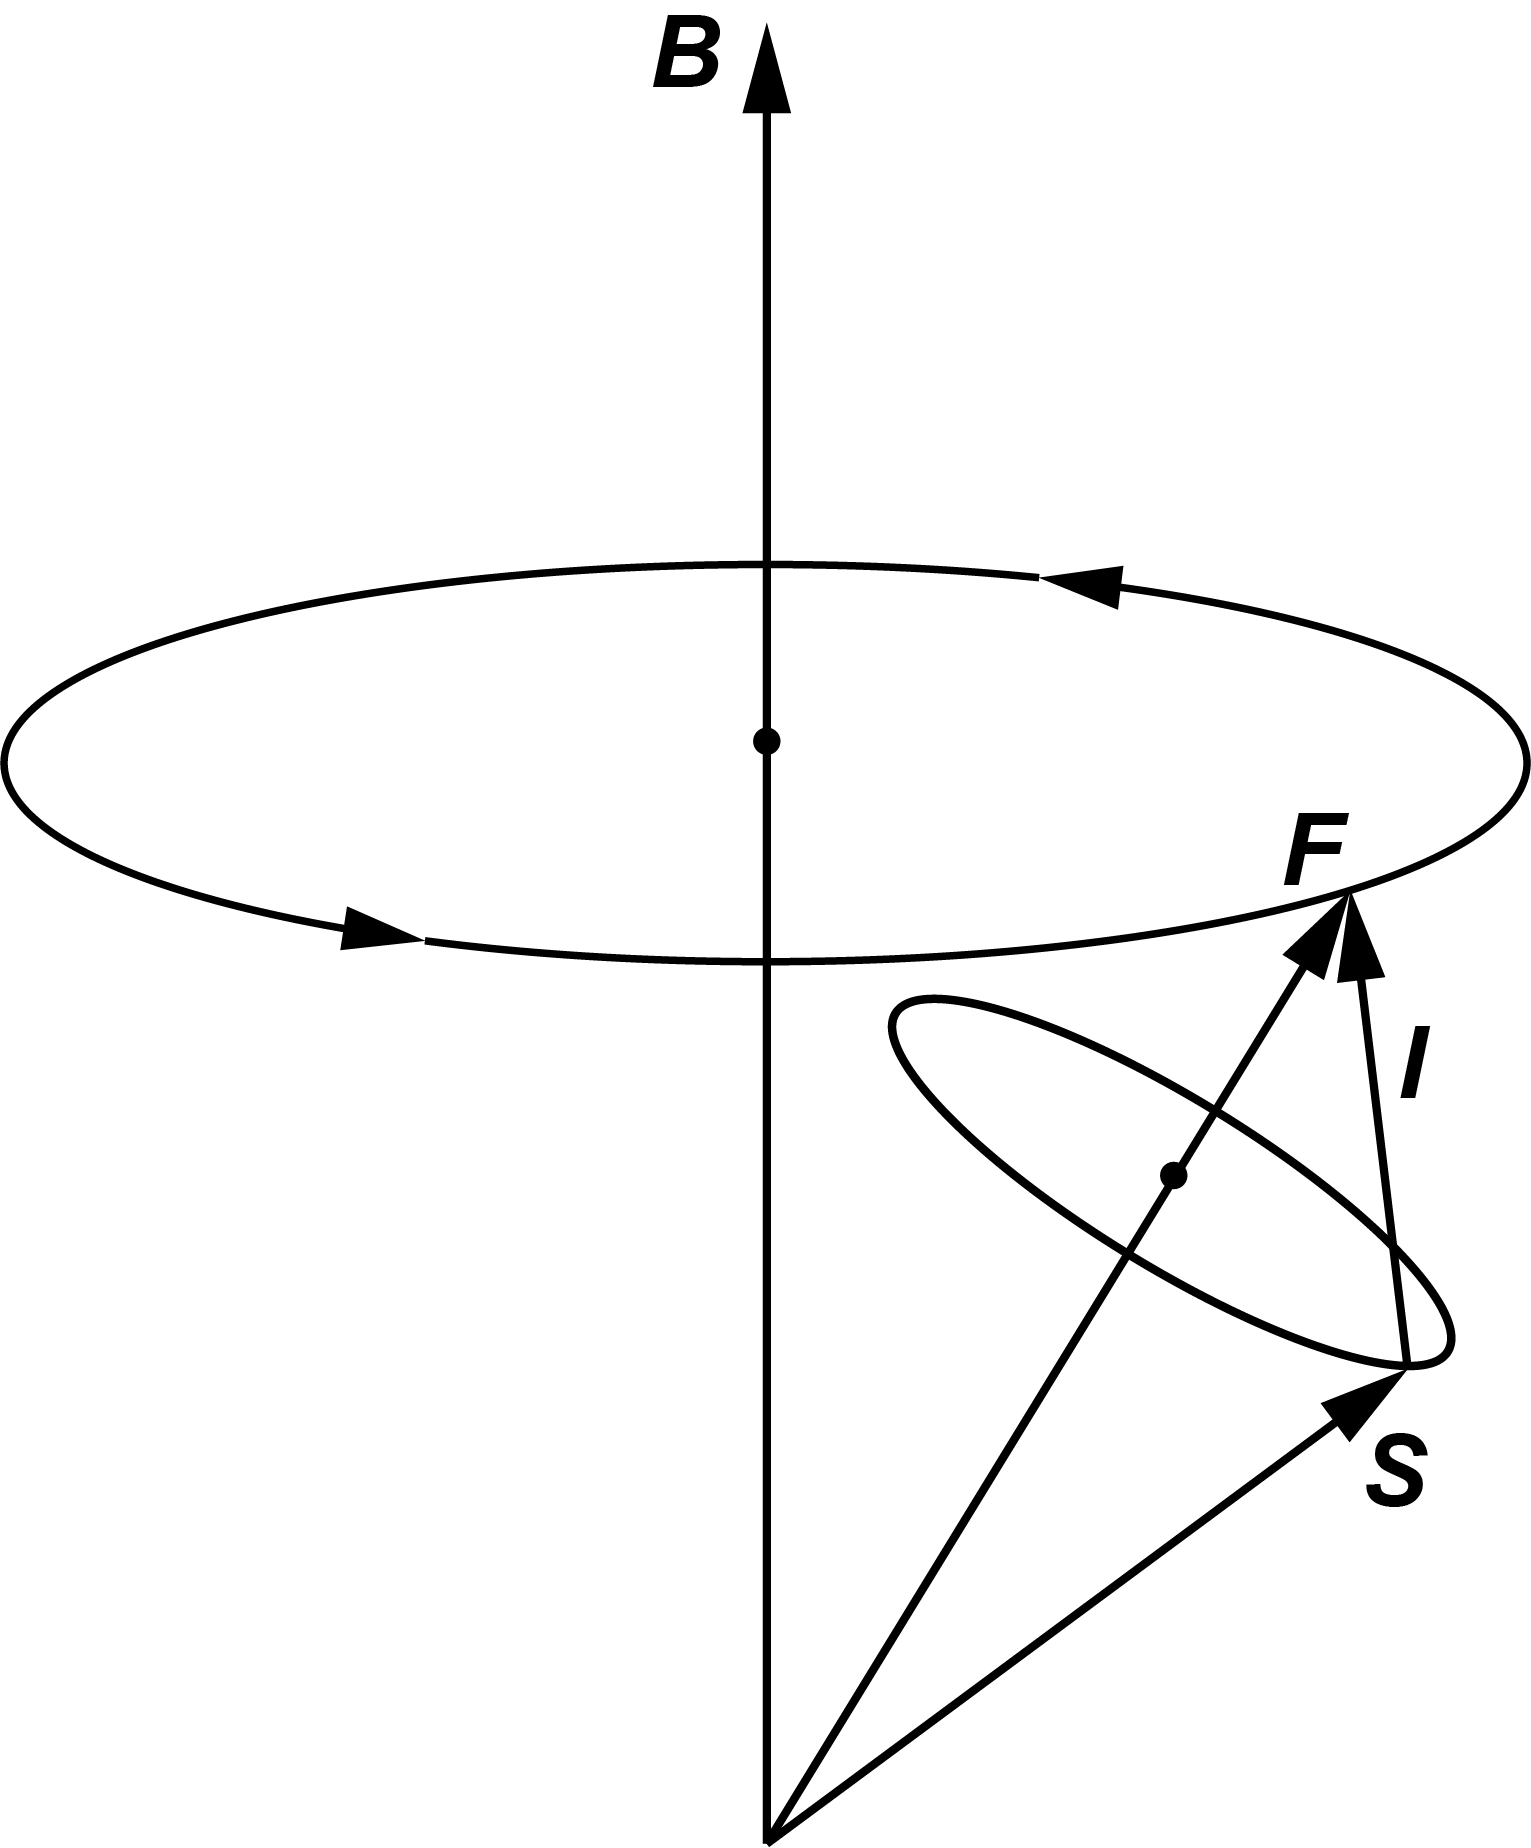
\includegraphics[width=0.4\textwidth]{WeakField.png}}
    \subfigure[强磁场下,$J$和$I$分别绕着磁场方向进动.]{
    \label{strong-field}
    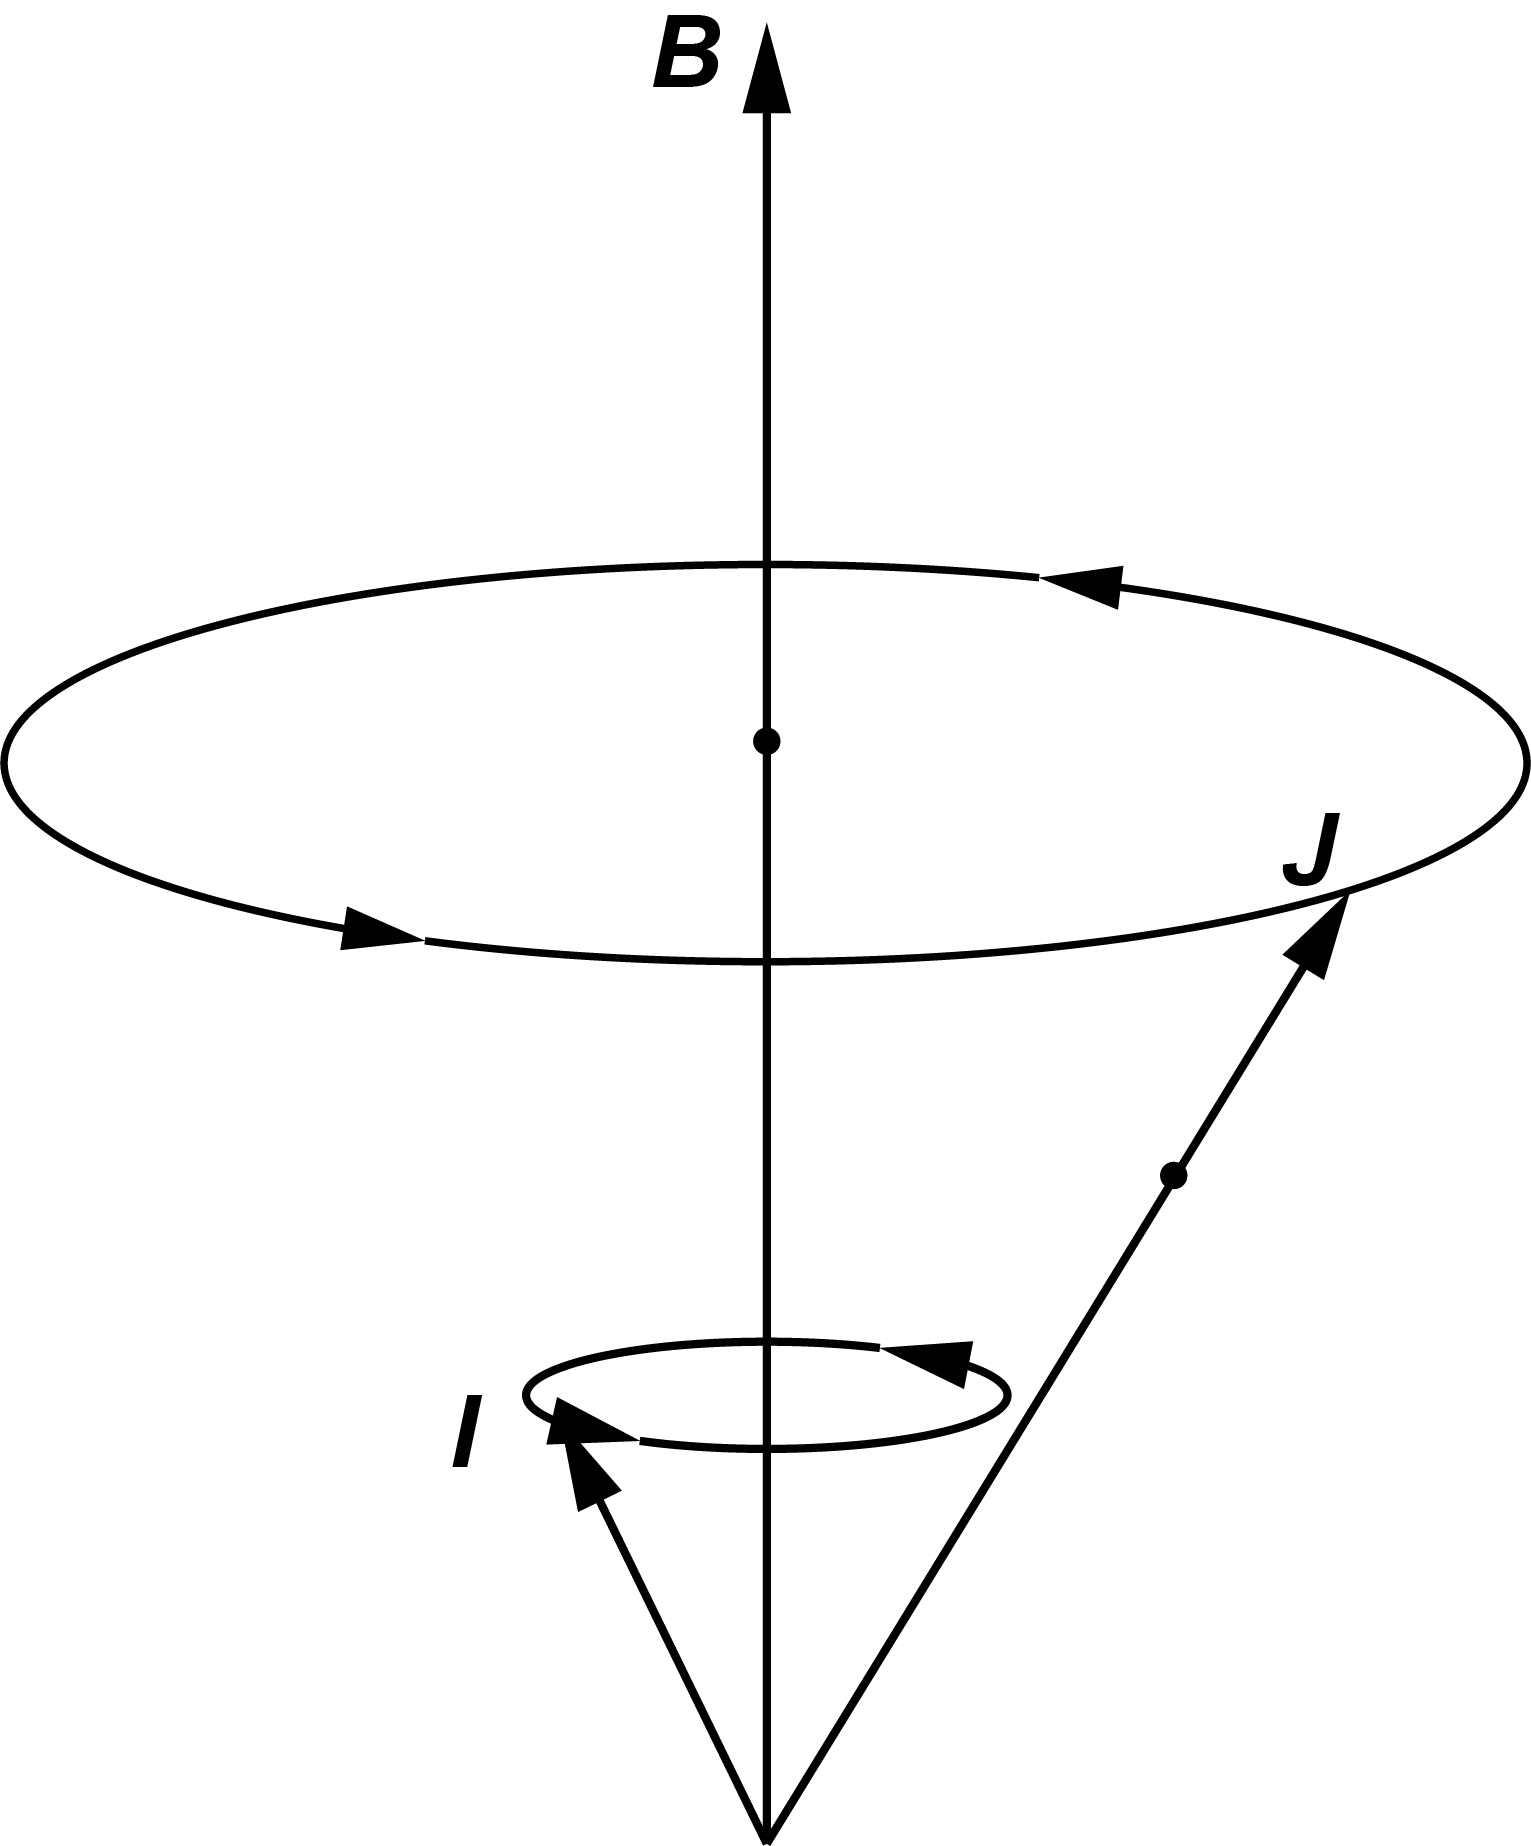
\includegraphics[width=0.4\textwidth]{StrongField.png}}
\end{figure}

在强磁场下,电子的总自旋$J$和核自旋$I$退耦合,两者分别绕磁场方向进动,如图\ref{strong-field},$J$和$I$在磁场方向的不同投影$m_J$和$m_I$造成了能级分裂:
\begin{align}
    E=(g_J\mu_Bm_J+g_I\mu_Nm_I)B,
\end{align}
其中玻尔磁子$\mu_B=\frac{\hbar e}{2m_e}$,核磁子$\mu_N=\frac{\hbar e}{2m_q}$,由于电子质量$m_e$比质子质量小三个数量级$m_p$,$\mu_B$比$\mu_N$大三个数量级,因此可略去上式中$m_I$对能级分裂的贡献,近似为
\begin{align}
    E=g_J\mu_Bm_JB.
\end{align}
其中$m_J$可取$-J,-J+1,\cdots,J-1,J$,故超精细能级结构中的每个能级都可分裂为$2J+1$个能级,如图\ref{energy-state-strong-field}所示. 这些能级之间的跃迁遵从选择定则:
\begin{gather}
    \Delta F=0,\pm 1,\\
    \Delta m_J=0,\pm 1.
\end{gather}

\begin{figure}[ht]
    \centering
    \subfigure[$^{85}$Rb]{
    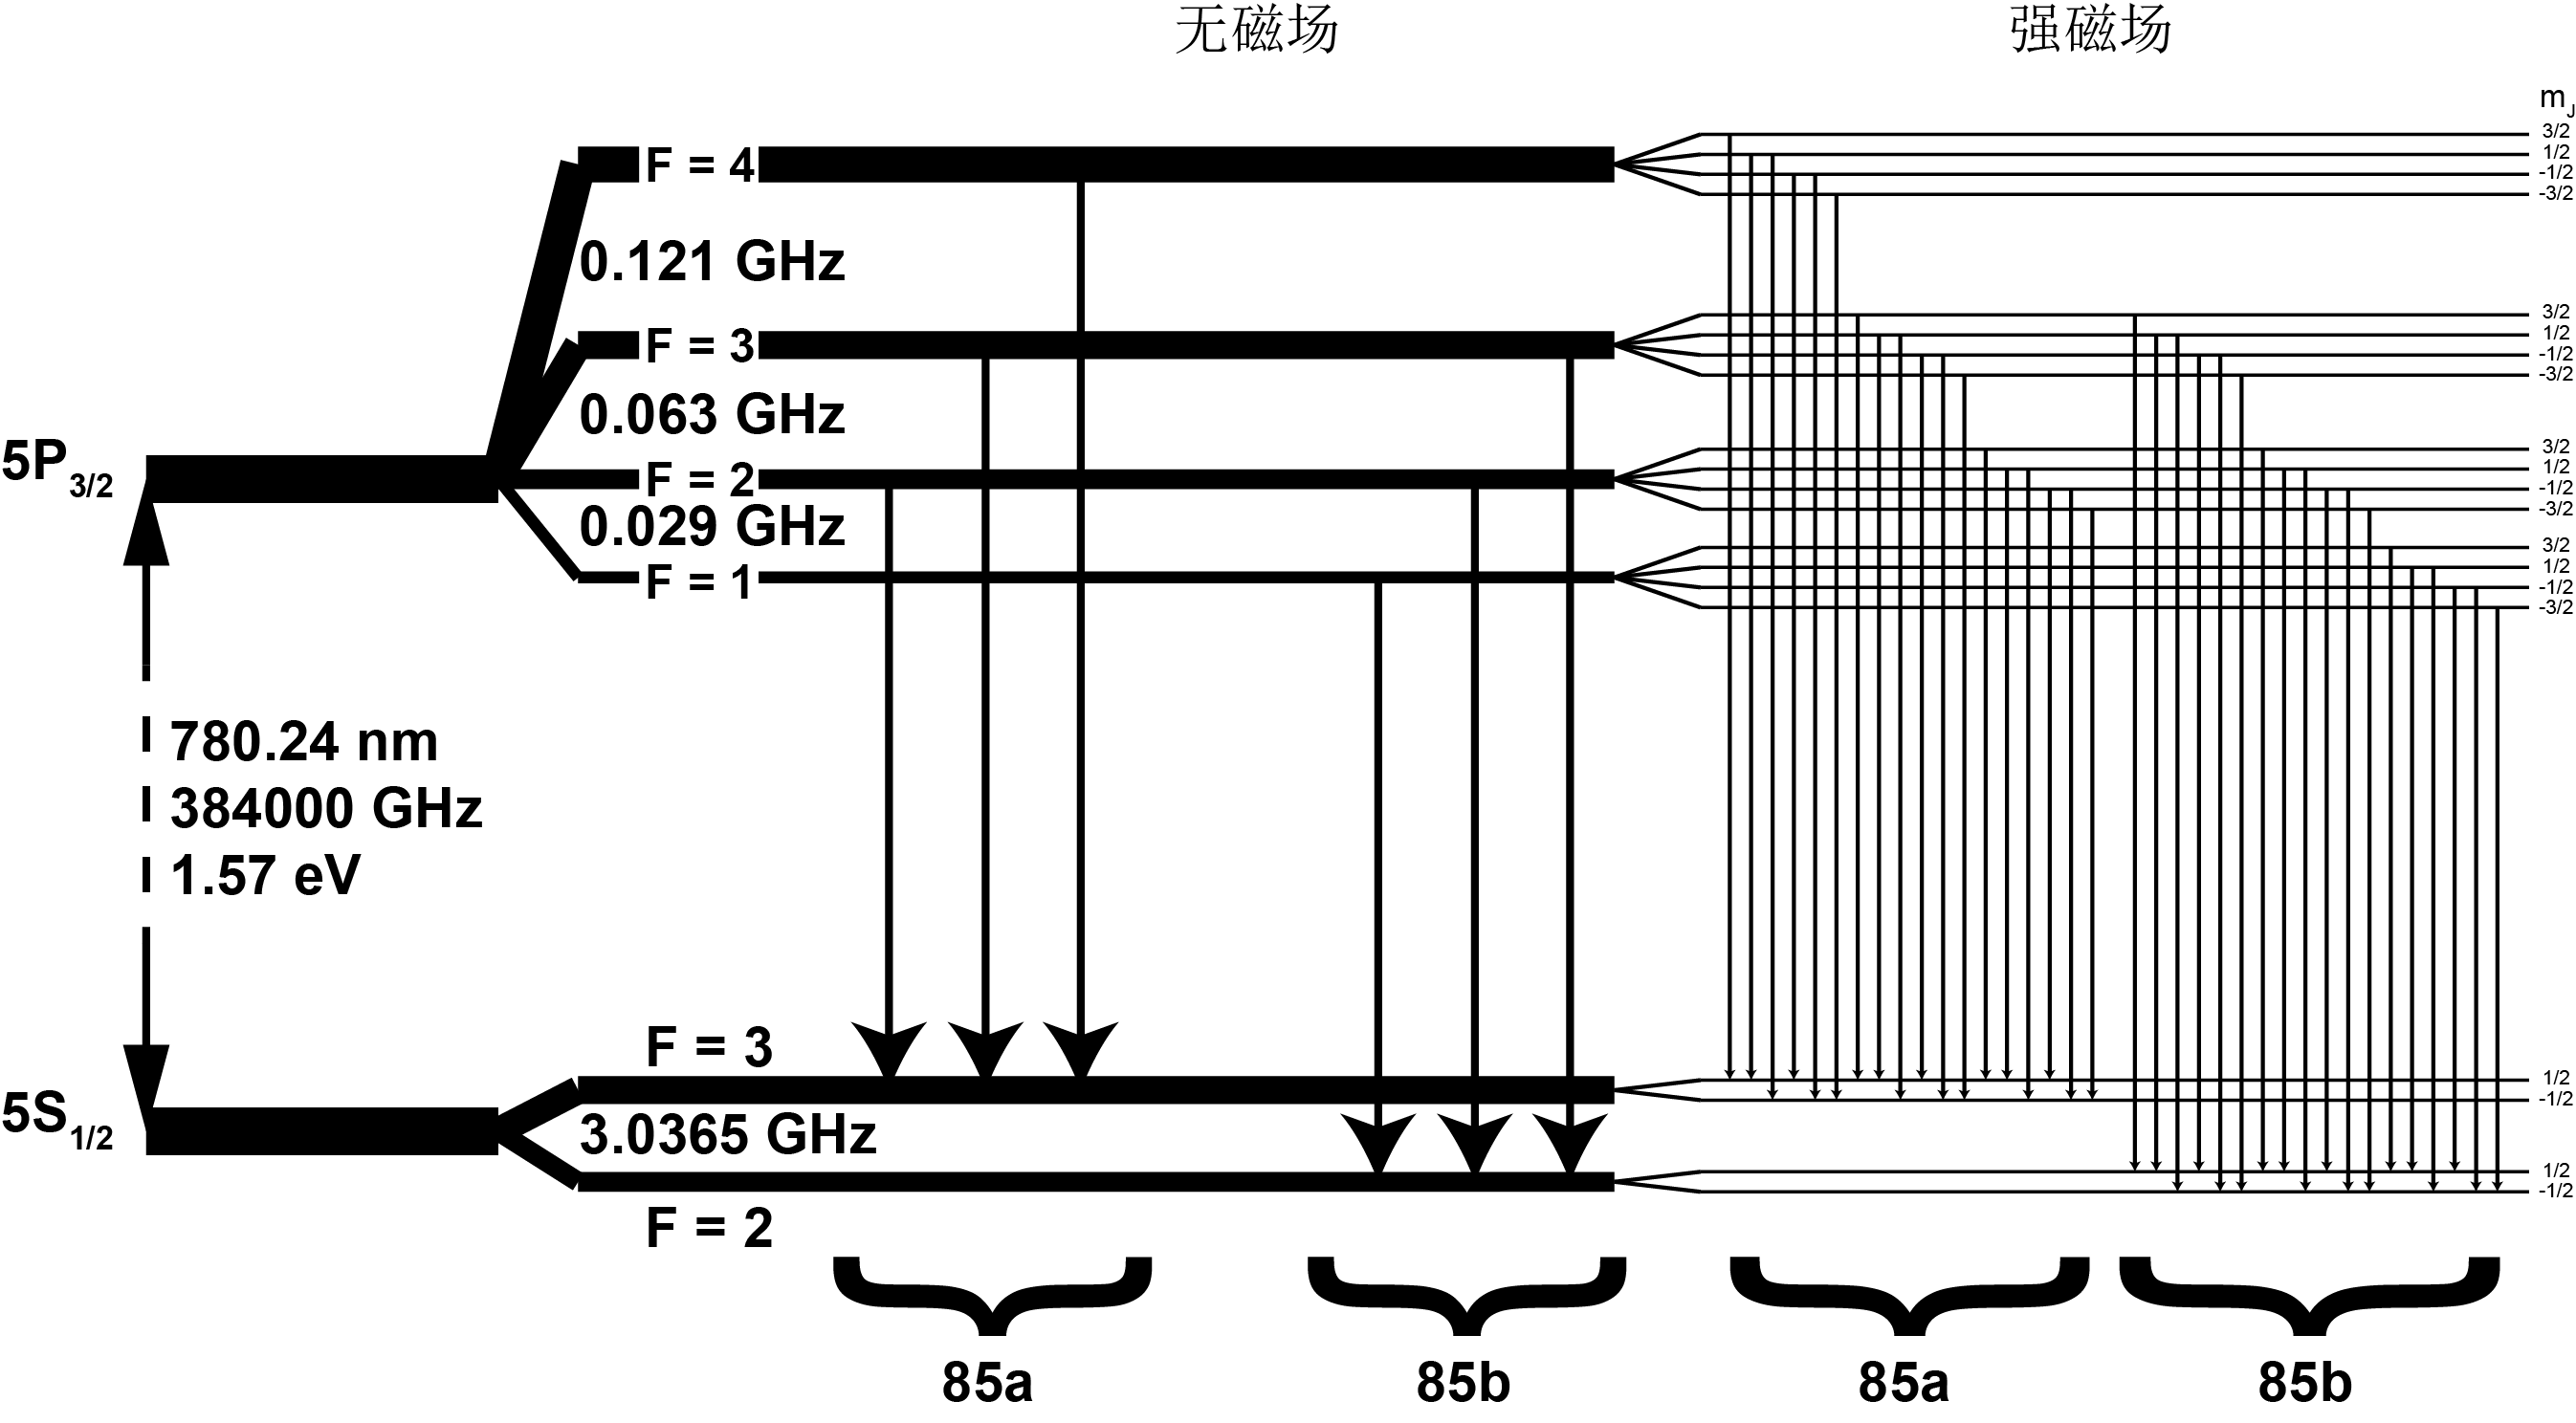
\includegraphics[width=0.8\textwidth]{EnergyState-85-StrongField.png}}
    \subfigure[$^{87}$Rb]{
    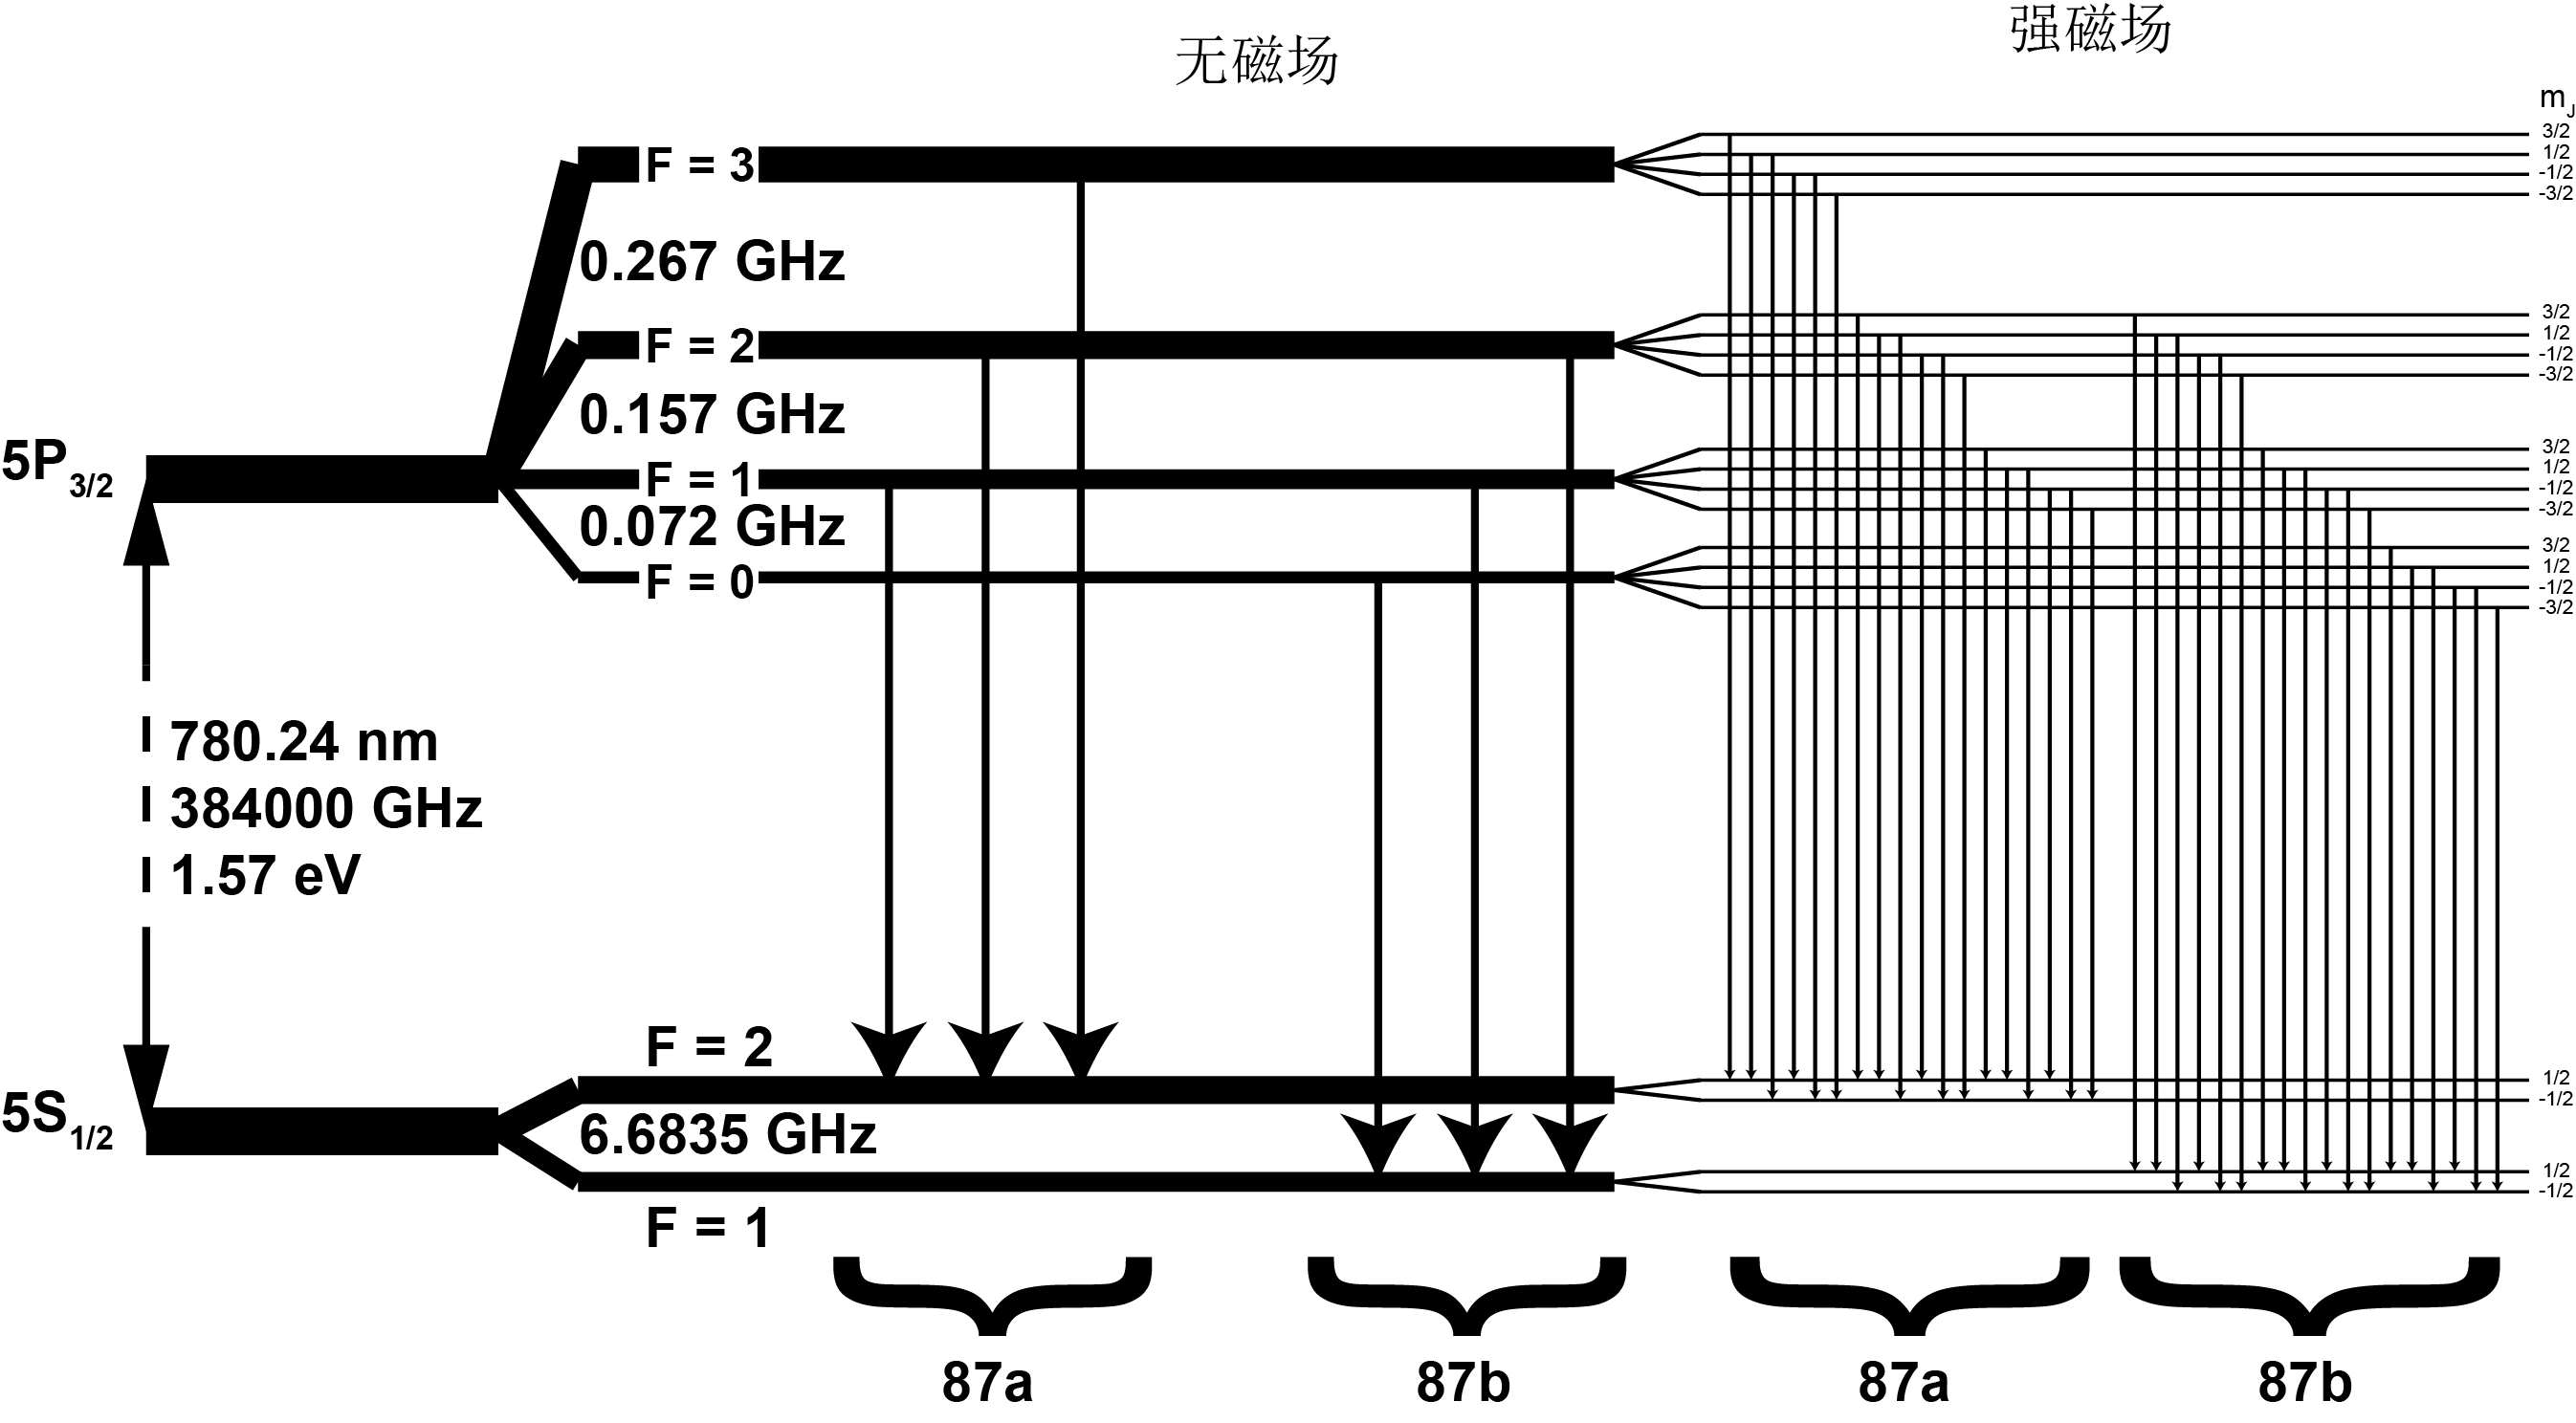
\includegraphics[width=0.8\textwidth]{EnergyState-87-StrongField.png}}
    \caption{在无磁场和强磁场下$^{85}$Rb和$^{87}$Rb的部分能级与允许的跃迁.(强磁场下,$F$大的能级分裂出的能级能量并非一定比$F$小的能级分裂出的能级更高,而是可能存在交叉,此处为清晰起见画出的分裂能级均没有交叉)}
    \label{energy-state-strong-field}
\end{figure}

本实验中所用的亥姆霍兹线圈可产生强度在$0\sim 10^{-2}$ T范围内连续变化的磁场,其最强磁场对应的能级分裂数量级$\sim 10^{-25}$ J$\sim 10^{-6}$ eV$\sim 10^{-1}$ GHz与超精细结构的能级分裂相当. 因此若实验仪器精度足够,可以观察到能级分裂情况在上述的无场、弱场、强场三种情况下的转换. 例如,对于$^{87}$b,若不考虑任何增宽,在无磁场下,应当有$3$条谱线,在弱场下,应当有$19$条谱线,在强场下,应当有$24$条谱线.

\subsection{光谱的展宽}

实际实验测得的光谱并非仅在能级跃迁对应的频率处存在信号,而是存在由有限的能级寿命导致的洛伦兹展宽和由热运动的原子的多普勒效应导致的多普勒增宽. 下面我们分别来讨论这两种增宽.

\subsubsection{自然增宽}

自然增宽来源于有限的能级寿命. 根据不确定性原理,能级的宽度和能级的平均寿命存在如下关系:
\begin{align}
    \Delta E\cdot\Delta t\geq\frac{\hbar}{2\pi}.
\end{align}
因此有限的能级寿命必然导致能级的增宽,从而反映在测得的谱线的增宽上. 利用一个半经典的模型,我们可以推导出这一增宽的线型:在单位时间内,原子从高能级跃迁至低能级并自发辐射的概率是常数,因此高能级上的原子数量是随着时间指数衰减的,单位时间内自发辐射的原子数也是随时间指数衰减的,从而辐射的电磁波强度也随着时间指数衰减,其电/磁场分量可表为
\begin{align}
    U(t)=U_0e^{-\frac{t}{2\tau}}e^{i2\pi\nu t},
\end{align}
其中$U_0$为电磁场的初始场强,$\tau$为高能级的寿命,也是光强衰减为原光强的$1/e$所需的时间,$\nu_0$表示两能级之间的共振频率.
利用傅里叶变换,辐射场可以展开为各个频率的简谐波的叠加
\begin{align}
    U(t)=\int_{-\infty}^{+\infty}u(\nu)e^{i2\pi\nu t}\,d\nu.
\end{align}
其中频率为$\nu$的电磁场分量为
\begin{align}
    u(\nu)=\int_{-\infty}^{+\infty}U(t)e^{-i2\pi\nu t}\,dt,
\end{align}
考虑到当$t<0$时,$U(t)=0$,上式可化为
\begin{align}
    u(\nu)=\int_0^{+\infty}U_0e^{-\frac{t}{2\tau}}e^{-i2\pi(\nu-\nu_0)t}\,dt=\frac{U_0}{i2\pi(\nu-\nu_0)+1/2\tau}.
\end{align}
光强正比于电磁场的平方,故圆频率为$\omega$的分量的光强具有如下的形式:
\begin{align}
    I(\omega)\propto\abs{u(\omega)}^2\propto\frac{1}{4\pi^2(\nu-\nu_0)^2+1/(2\tau)^2}.
\end{align}
归一化后可得相对光强(单位频率范围内光强在总光强中的占比):
\begin{align}
    f_N(\nu)=\frac{1/\tau}{4\pi^2(\nu-\nu_0)^2+(1/2\tau)^2}=\frac{\Delta\nu_N/2\pi}{(\nu-\nu_0)^2+(\Delta\nu_N/2)^2},
\end{align}
其中半高宽\
\begin{align}
    \label{nature-width}
    \Delta\nu_N=\frac{1}{2\pi\tau}.
\end{align}
此即自然增宽的光谱线型函数,为一洛伦兹型函数. 一般原子激发态的平均寿命数量级$\sim 10^{-5}-10^{-8}$ s,故自然增宽的数量级大致在$10^{-4}\sim 10^{-1}$ GHz范围内.

\subsubsection{多普勒增宽}

多普勒增宽来自于介质中热运动的原子的多普勒效应. 常温下气体中原子的运动遵循麦克斯韦速度分布律,$z$方向速度分量在$v_z\sim v_z+dv_z$范围内的原子数在总原子数中的占比为
\begin{align}
    \frac{dn_z}{n}=\left(\frac{m}{2\pi k_BT}\right)^{1/2}e^{-\frac{mv_z^2}{2k_BT}}\,dv_z,
\end{align}
其中$m$为一个原子的质量,$k_B$为玻尔兹曼常数,$T$为热力学温度. 根据多普勒效应,这部分原子所吸收和辐射的光子频率为
\begin{align}
    \nu=\left(1+\frac{v_z}{c}\right)\nu_0,
\end{align}
其中$\nu_0$为静止原子的能级跃迁频率. 这部分原子吸收或辐射的光强在总光强中的占比即为对应的原子数占比
\begin{align}
    f_D(\nu)\,d\nu=\frac{dn_z}{n}=\left(\frac{m}{2\pi k_BT}\right)^{1/2}\exp\left[-\frac{mc^2(\nu-\nu_0)^2}{2k_BT\nu_0^2}\right]\frac{c}{\nu_0}\,d\nu,
\end{align}
故相对光强为
\begin{align}
    \nonumber f_D(\nu)=&\left(\frac{m}{2\pi k_BT}\right)^{1/2}\exp\left[-\frac{mc^2(\nu-\nu_0)^2}{2k_BT\nu_0^2}\right]\frac{c}{\nu_0}\\
    =&\frac{2}{\Delta\nu_D}\left(\frac{\ln 2}{\pi}\right)^{1/2}\exp\left\{-\left[4\ln 2\left(\frac{\nu-\nu_0}{\Delta\nu_D}\right)^2\right]\right\},
\end{align}
其中半高宽
\begin{align}
    \label{Doppler-width}
    \Delta\nu_D=2\nu_0\left(\frac{2k_BT}{mc^2}\ln 2\right)^{1/2}.
\end{align}
此即多普勒增宽的光谱线型函数,为一高斯型函数. 将式\ref{Doppler-width}中各常数代入可得
\begin{align}
    \Delta\nu_D=7.16\times 10^{-7}\sqrt{T/\mu_{\text{mol}}}\nu_0,
\end{align}
其中$\mu_{\text{mol}}$为原子量,以铷原子为例,$\mu_{\text{mol}}=85.5$,$^2$P$_{3/2}$态和$^2$S$_{1/2}$态间跃迁频率为$384000$ GHz,在常温($\sim 300$ K)下,其多普勒增宽$\sim 0.5$ GHz,远大于自然增宽,故光谱的增宽以多普勒增宽为主导.

\subsubsection{综合增宽}

实际的光谱增宽同时来自上述两种增宽机制的综合贡献,如图\ref{Broadening}所示:热运动的原子的速度满足高斯分布,而处于各个速度的原子各自辐射出指数衰减的电磁波,因此处于各个速度的原子都对总光谱贡献洛伦兹线型的子光谱(图中红线),这些子光谱按照高斯型的权重(图中绿线)叠加成总光谱(图中蓝线),总光谱线型函数为自然增宽线型函数和多普勒增宽线型函数的卷积:
\begin{align}
    f(\nu)=\int_{-\infty}^{+\infty}f_L(\nu')f_D(\nu-\nu')\,d\nu'.
\end{align}
这一线型称为Voigt线型.

\begin{figure}[h]
    \centering
    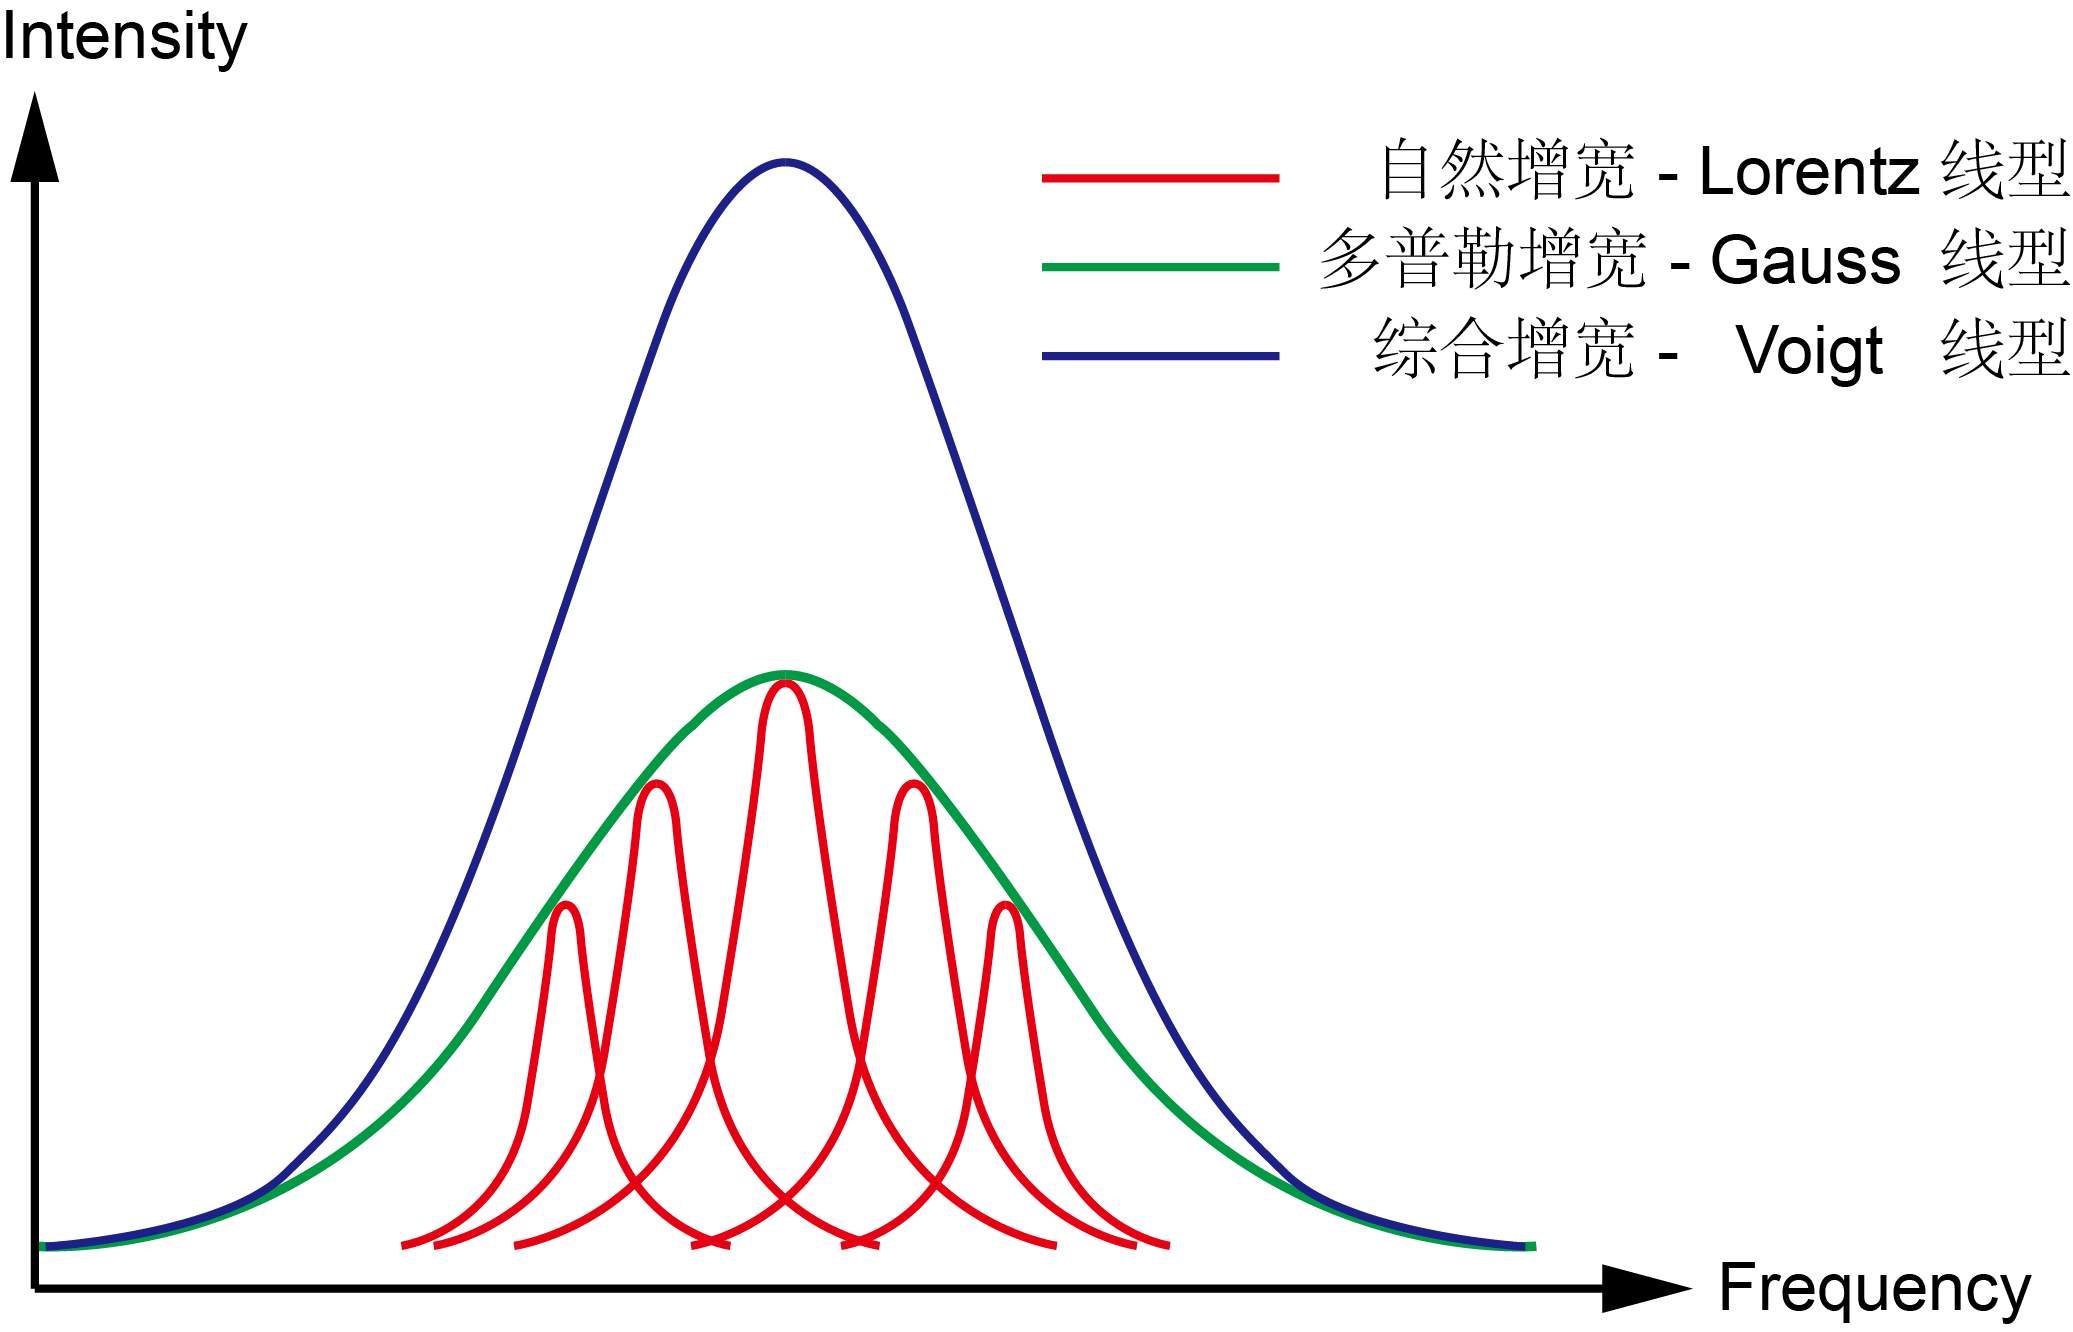
\includegraphics[width=.6\textwidth]{Broadening.png}
    \caption{综合增宽机制示意图:各洛伦兹线型子光谱以高斯线型权重叠加成Voigt线型总光谱.}
    \label{Broadening}
\end{figure}

\subsection{饱和吸收光谱}

为了在常温下测得待测介质的超精细结构,我们需要消除多普勒增宽的影响,一个有效的方法是采用饱和吸收光谱技术. 饱和吸收光谱是将同频率的、展宽远小于介质多普勒增宽的一束泵浦光和和一束探测光从同一条路径、两个相反的方向入射介质,通过扫描两束激光的频率而测得的探测光光谱.

\subsubsection{饱和吸收光谱的基本原理}

由于多普勒效应,沿着光路具有速度分量的原子感受到的泵浦光和探测光具有不同的频率,而沿着光路速度分量为零的原子感受到到的泵浦光和探测光具有相同的频率. 如图\ref{SAS-1}所示,假设泵浦光从左入射介质,而探测光从右入射介质,两束激光光路重合. 若仅考虑原子在能量差为$h\nu$的两个能级之间的跃迁,当泵浦光和探测光的频率与原子的共振频率失谐,为$(\nu-\delta\nu)$,则从左入射介质的泵浦光仅激发以$\frac{\delta\nu}{\nu_0}c$向左运动的原子,吸收从右传入射介质的探测光的则是以$\frac{\delta\nu}{\nu_0}c$向左运动的原子,因此泵浦光不影响探测光的吸收强度,光谱强度与无饱和吸收的光谱相等;若泵浦光和探测光与原子在两个能级间的跃迁共振,即其频率为$\nu_0$,则两束光均与静止的原子发生相互作用,由于较强的泵浦光激发将近半数的原子激发至激发态,能吸收探测光的基态原子数量就相应减少,因此吸收强度较无饱和吸收的更小,饱和吸收光谱在$\nu_0$处产生了一个“烧孔”. 由于在烧孔处,因此仅当激光的频率扫描到静止原子的激发频率,. 因此饱和吸收光谱会在原子的共振频率处产生烧孔,这些烧孔的线型即为自然增宽.

\begin{figure}[h]
    \centering
    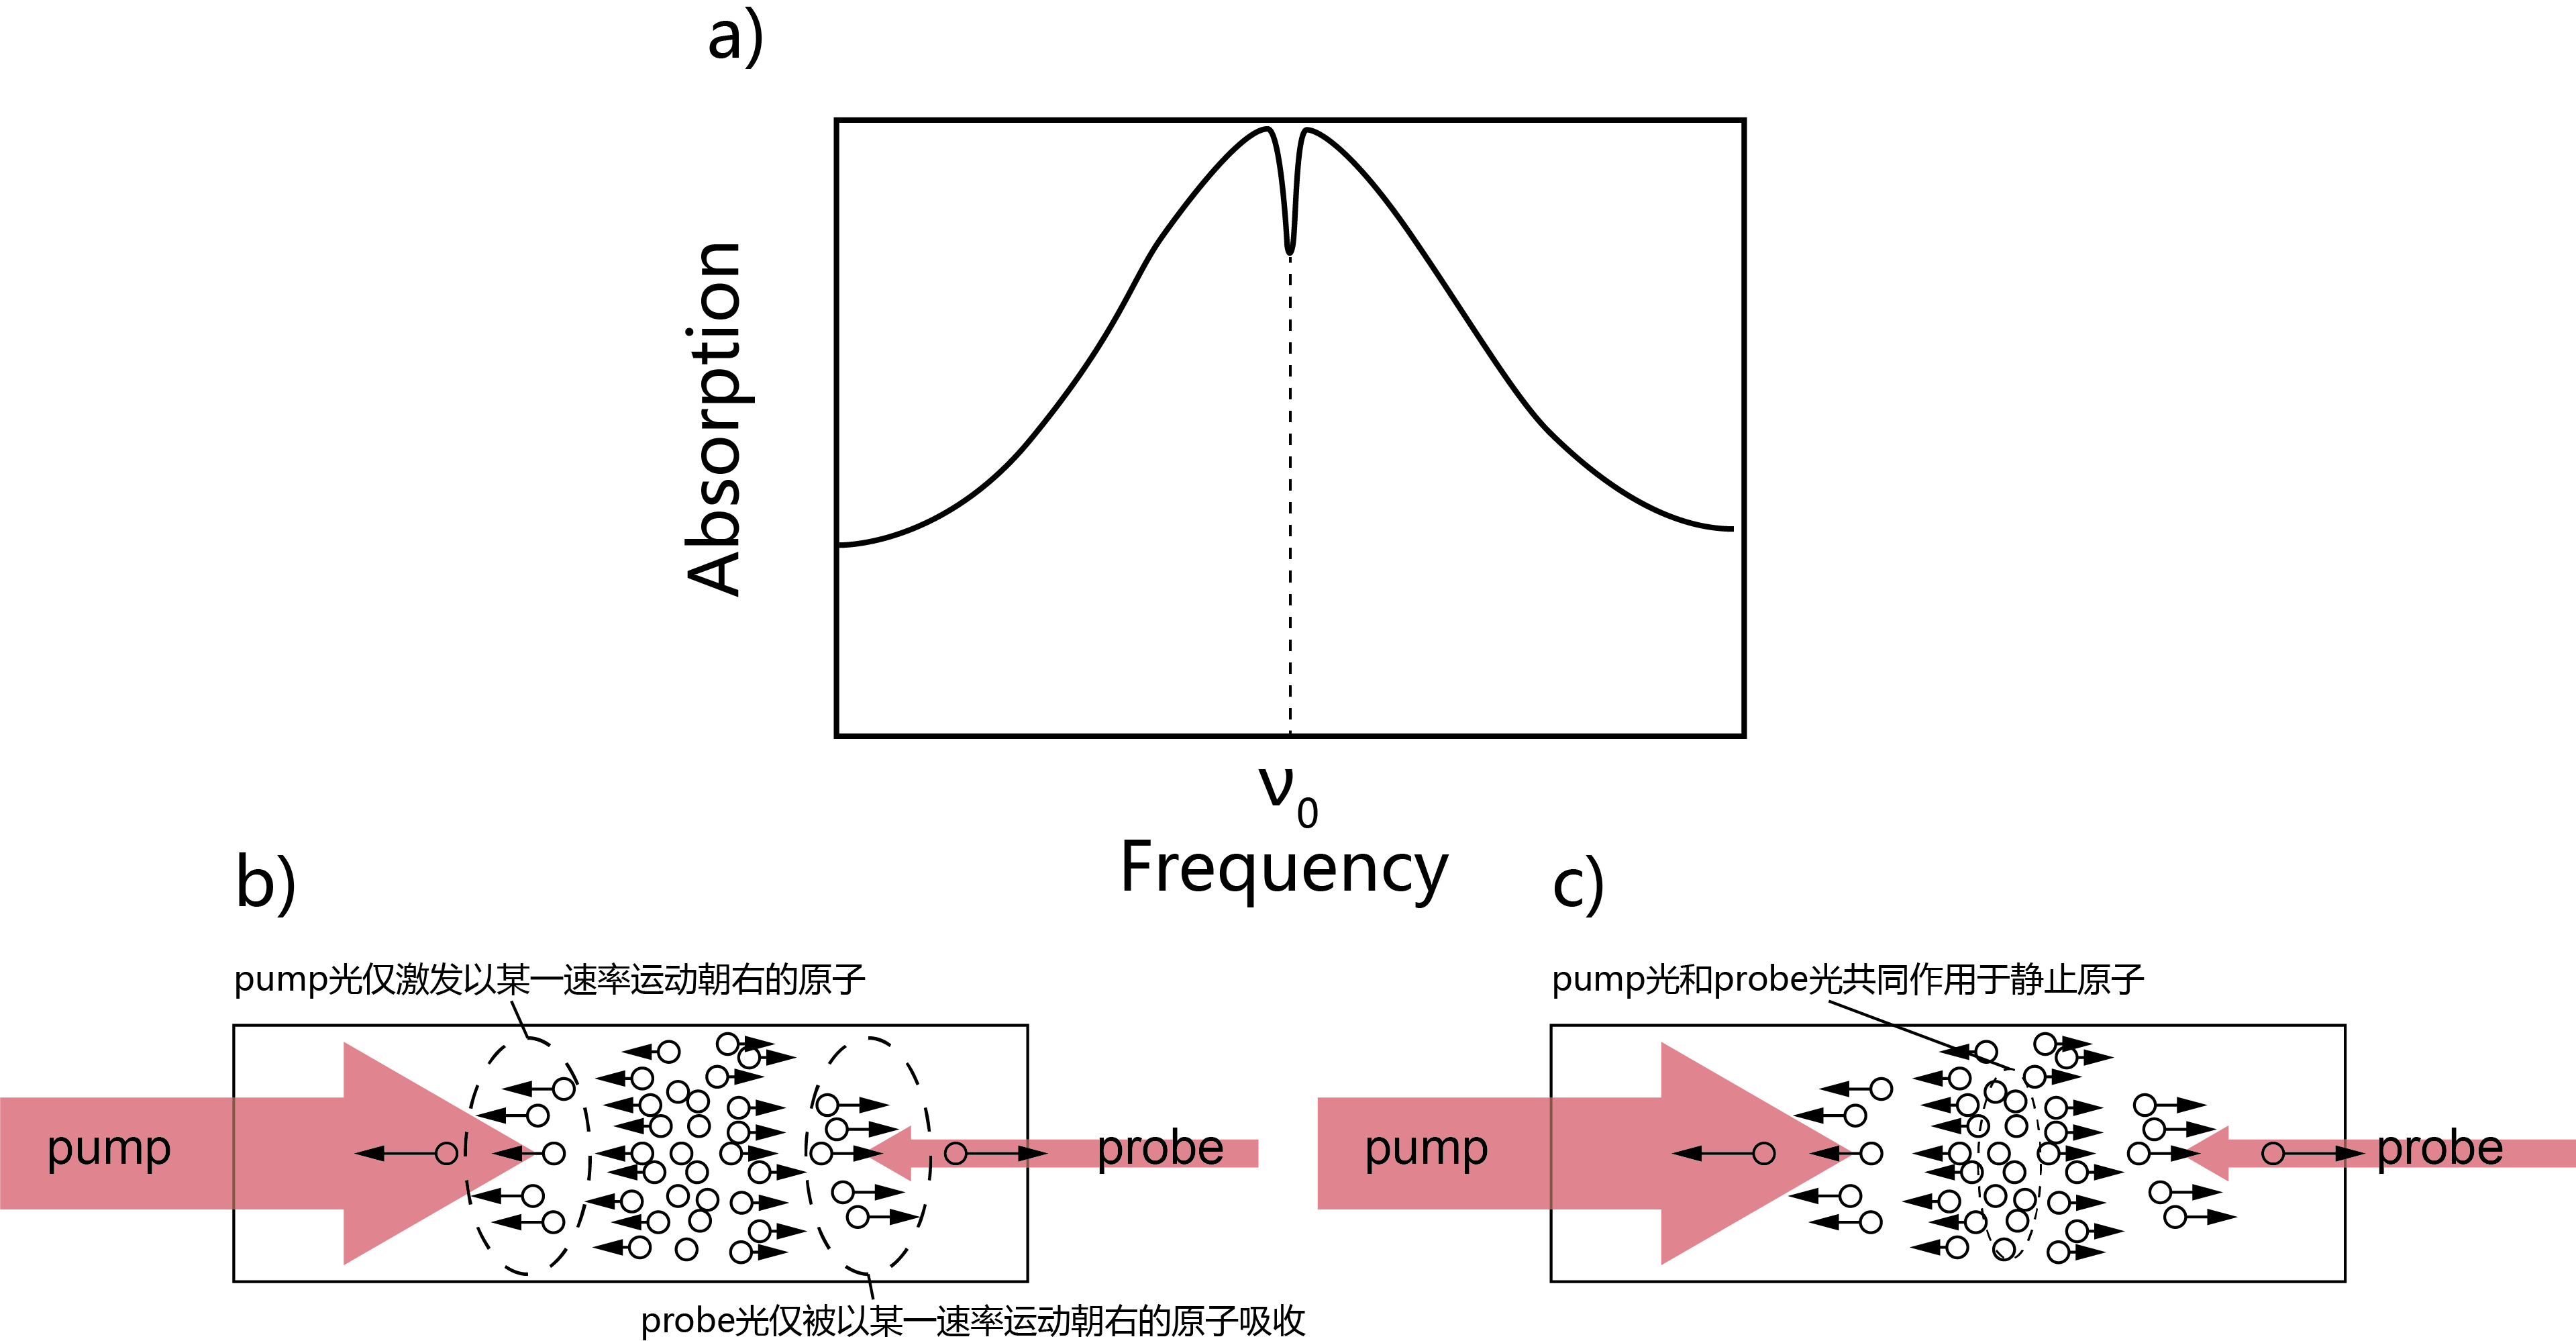
\includegraphics[width=.9\textwidth]{SAS-1.png}
    \caption{饱和吸收光谱原理示意图. (a) 饱和吸收光谱理论线型,(b) 当入射激光频率略小于跃迁频率,激光与气体中原子的作用机制,(c) 当入射光频率等于跃迁频率时,激光与气体中原子的作用机制.}
    \label{SAS-1}
\end{figure}

\subsubsection{交叉共振现象}

实际实验中测得饱和吸收光谱不仅在原子能级跃迁的共振频率处存在烧孔,在任意两个跃迁频率$\nu_1$和$\nu_2$的中点$(\nu_1+\nu_2)/2$处也存在着烧孔,这称为交叉共振(crossover resonance).

交叉共振现象是由原子不同能级跃迁的相互影响造成的. 如图\ref{SAS-2}(a)所示,以一个V型的三能级系统为例,原子可以由基态$0$吸收$h\nu_1$的能量向激发态$1$跃迁,或吸收$h\nu_2$的能量向激发态$2$跃迁,由于选择定则的限制,原子不能在两个激发态之间跃迁. 如图\ref{SAS-2}(b)所示,当入射的泵浦光和探测光的频率为$(\nu_1+\nu_2)/2$时,对于以速率$(\nu_2-\nu_1)c/2(\nu_1+\nu_2)$向左运动的原子,其感受到泵浦光的频率为$\nu_2$而感受到探测光的频率为$\nu_1$,故这部分原子大部分被泵浦光激发至$2$态,而对探测光的吸收较无泵浦光时更弱,而对于以速率$(\nu_2-\nu_1)c/2(\nu_1+\nu_2)$现有运动的原子,其感受到泵浦光的频率为$\nu_1$而感受到探测光的频率为$\nu_2$,故这部分原子大部分被泵浦光激发至$1$态,而对探测光的吸收较无泵浦光时更弱,因此饱和吸收光谱在$(\nu_1+\nu_2)/2$处产生一个额外的烧孔,如图\ref{SAS-2}(c)所示.

交叉共振处的吸收强度并非总是降低. 对于$\Lambda$型的三能级系统,我们可以同理预测,交叉共振处存在一个峰,而非一个烧孔,如图所示.

因为交叉共振的烧孔由两批不同速度的原子贡献,因此其烧孔大小往往较原子原有跃迁频率处的烧孔要大.

\begin{figure}[h]
    \centering
    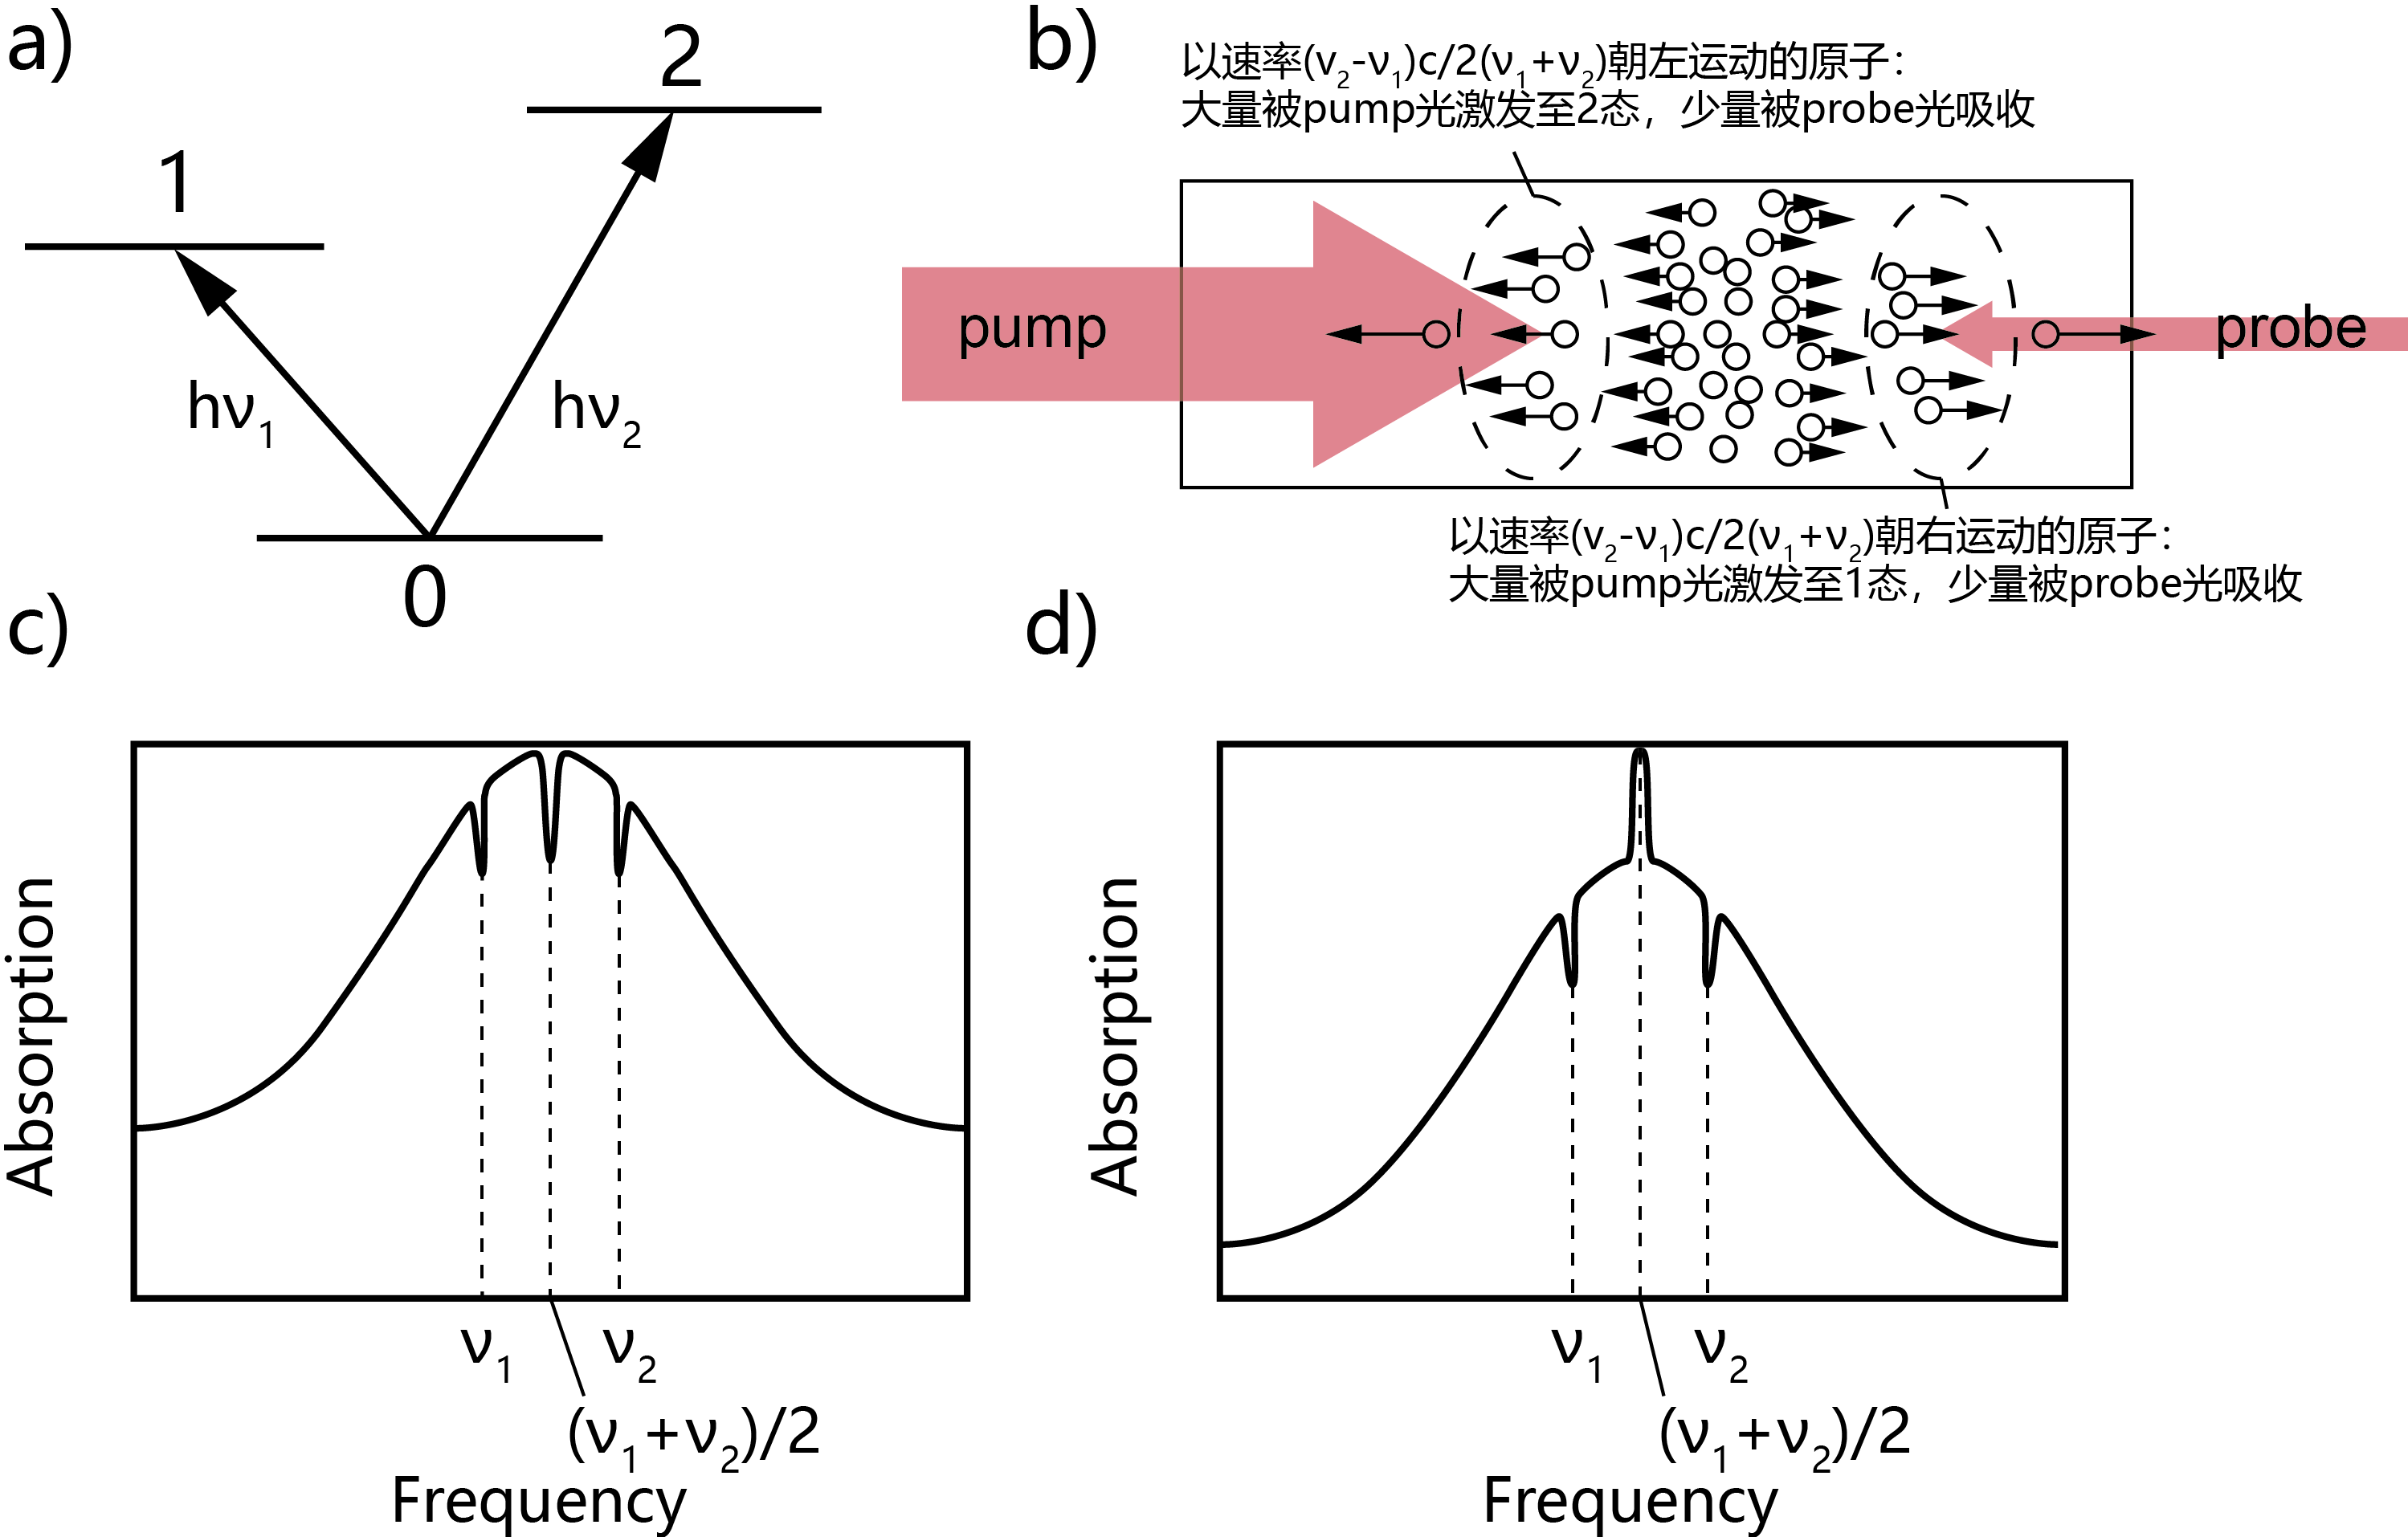
\includegraphics[width=.8\textwidth]{SAS-2.png}
    \caption{交叉共振现象示意图. (a) V型三能级系统,(b) 当入射激光频率为$(\nu_1+\nu_2)/2$时,激光与气体中原子的作用机制,(c) V型三能级系统的饱和吸收光谱理论线型,(d) $\Lambda$型三能级系统的饱和吸收光谱理论线型.}
    \label{SAS-2}
\end{figure}

\section{实验测量}

\subsection{实验装置和方法}

我们的实验装置如图\ref{light-path}所示. 由外腔反馈二极管激光器发出的激光,经过中性滤光片衰减后被一楔形10-90分束器分为三束:其中光强占总光强$10\%$的两束反射光,分别作为探测光和参考光入射温度维持在$50^{\circ}$C的Rb蒸汽吸收室,最终分别被两个光电二极管探测器接收;光强占总光强$90\%$的透射光经过两面反射镜反射后,被一50-50分束器分为两束,反射的一束作为泵浦光以与探测光路径重合的路径反向入射Rb吸收室实现饱和吸收,透射的另一束经法布里-珀罗腔选频,最终被一光电二极管探测器接收. 法布里-珀罗腔前置一偏振片和一1/4波片,以实现该路光束的单向传播,防止光线反射回激光器中影响激光器稳定工作.

用三角波调制激光器的激励电流和激光器外腔的压电陶瓷,以实现激光频率的连续扫描. \textcircled{\scriptsize{12}}号探测器测得饱和吸收光谱,\textcircled{\scriptsize{13}}号探测器测得无饱和的吸收光谱,\textcircled{\scriptsize{13}}号探测器可以测得周期性的信号,可以用来作为光谱的频率参考,方便后续数据处理时修正示波器时间分辨的误差和激光器的频率漂移.

\begin{figure}[ht]
    \centering
    \includegraphics[width=.8\columnwidth]{LightPath.png}
    \caption{实验装置: \textcircled{\footnotesize{1}}——外腔反馈二极管激光器,Sanyo DL-7140-201A,最大功率$70$ mW,中心波长$785$ nm;\textcircled{\footnotesize{2}}——中性滤光片,Thor Labs NE10B,透过率$15\%$@$780$ nm;\textcircled{\footnotesize{3}}——10-90分束器,Red Optronics RWP 10X,楔形,$1^{\circ}$,\textcircled{\footnotesize{4}}\textcircled{\footnotesize{5}}——平面反射镜,Thor Labs ME1-G01,\textcircled{\footnotesize{6}} —— 50-50分束器,Edmunds Optics Y45-853,\textcircled{\footnotesize{7}}——偏振片,American Polarizer(3M) 98-0440-0968-0,\textcircled{\footnotesize{8}}——1/4波片,American Polarizer(3M) 98-0440-1064-7,\textcircled{\footnotesize{9}}——法布里-珀罗腔,工作波长范围$780\pm 40$ nm,\textcircled{\scriptsize{10}}——Rb蒸汽吸收室,\textcircled{\scriptsize{11}}——亥姆霍兹线圈对,半径$87.4$ mm,$320$匝,\textcircled{\scriptsize{12}}\textcircled{\scriptsize{13}}\textcircled{\scriptsize{14}}——光二极管探测器,PDB-C108. 红色箭头表示各路光束的传播方向.}
    \label{light-path}
\end{figure}

\subsection{实验结果和讨论}

实验测得在无磁场下铷蒸汽吸收光谱(参考光光谱)如图\ref{Absorption-noField}所示. 利用Voigt峰形对该光谱进行多峰拟合,得到$85$a,$87$a的峰面积之比为$0.02197:0.00754=74.4\%:25.6\%$,此即铷蒸汽吸收室中两种同位素$^{87}$Rb和$^{85}$Rb的占比,与其在自然界中的丰度比值$72.17\%:27.83\%$相近.

拟合还得到了$\Delta\nu_D=0.68502$ GHz,代入式\eqref{Doppler-width}中可得气体温度为$T=531$ K. 这一温度高于铷蒸汽吸收室的设定温度($323$ K),这是因为吸收光谱中的每个峰实际上都包含了超精细结构中的三个峰,超精细结构的能级分裂在$10^{-1}$ GHz量级,与$\Delta\nu_D$在同一量级,因此计算得到的气体温度与实际值存在一定的偏差.

\begin{figure}[h]
    \centering
    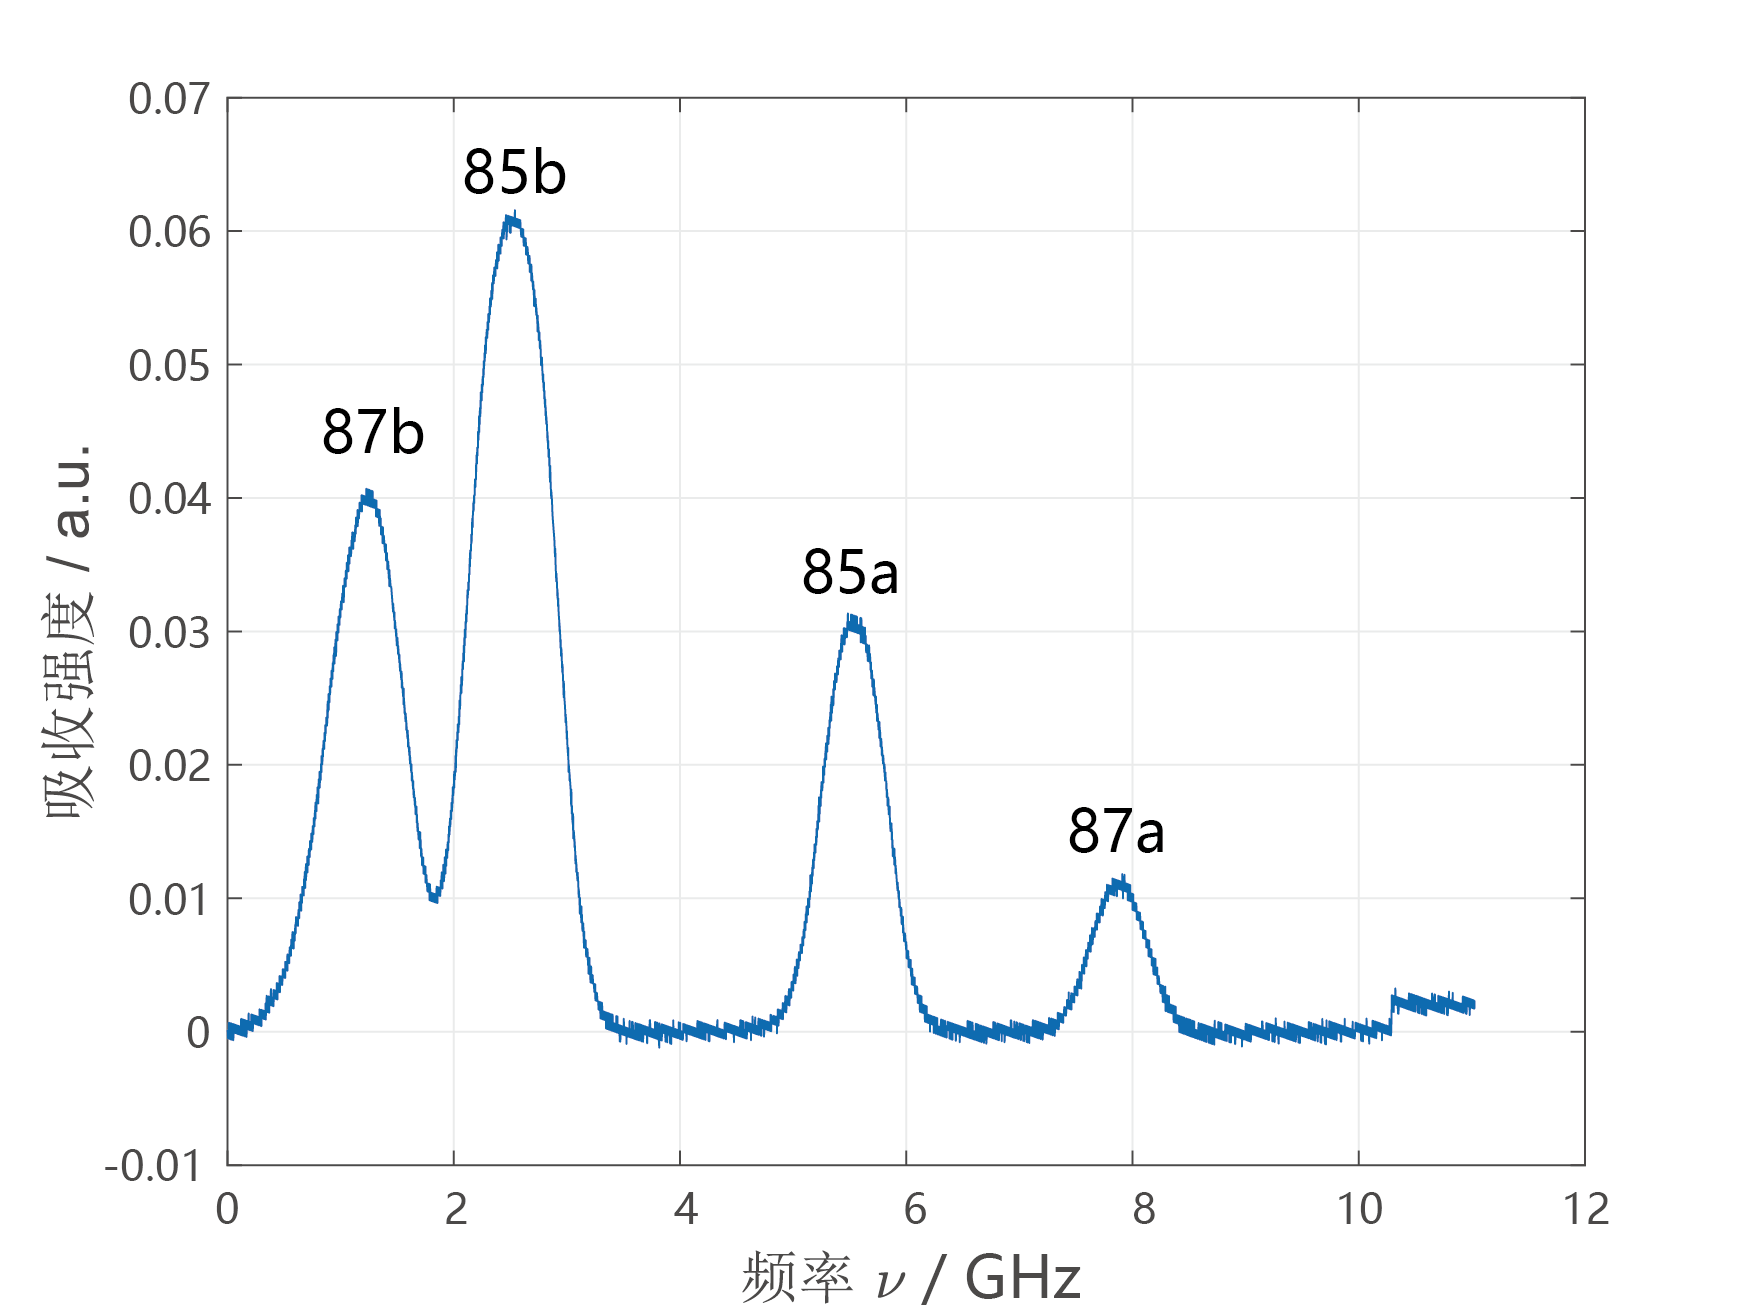
\includegraphics[width=.5\textwidth]{Absorption-noField.png}
    \caption{无磁场下铷蒸汽吸收光谱(横坐标由已知的$87$a和$87$b之间的频率差推得,已扣除由于激光强度改变的线性背底).}
    \label{Absorption-noField}
\end{figure}

将无磁场下的参考光信号与探测光的信号以一定比例相减,得到饱和吸收光谱中烧孔的谱线,如图\ref{holeburning-noField}所示. 其中我们找出了$87$b和$85$b各自包含的三条谱线的频率. $85$b的三个烧孔的两两间距为$0.03236$ GHz和$0.06611$ GHz,这三个烧孔应该是图\ref{energy-state}中$85$b对应的三个跃迁的交叉共振,理论上这两个间距应为 $\frac{0.063}{2}\text{GHz}=0.0315$ GHz和 $\frac{0.121}{2}\text{GHz}=0.0605$ GHz. $87$b的三个烧孔的两两间距分别为$0.09737$ GHz和$0.15138$ GHz,这三个烧孔应该是图\ref{energy-state}中$87$b对应的三个跃迁的交叉共振,理论上这两个间距应为 $\frac{0.157}{2}\text{GHz}=0.0785$ GHz和 $\frac{0.287}{2}\text{GHz}=1.335$GHz.

\begin{figure}[h]
    \centering
    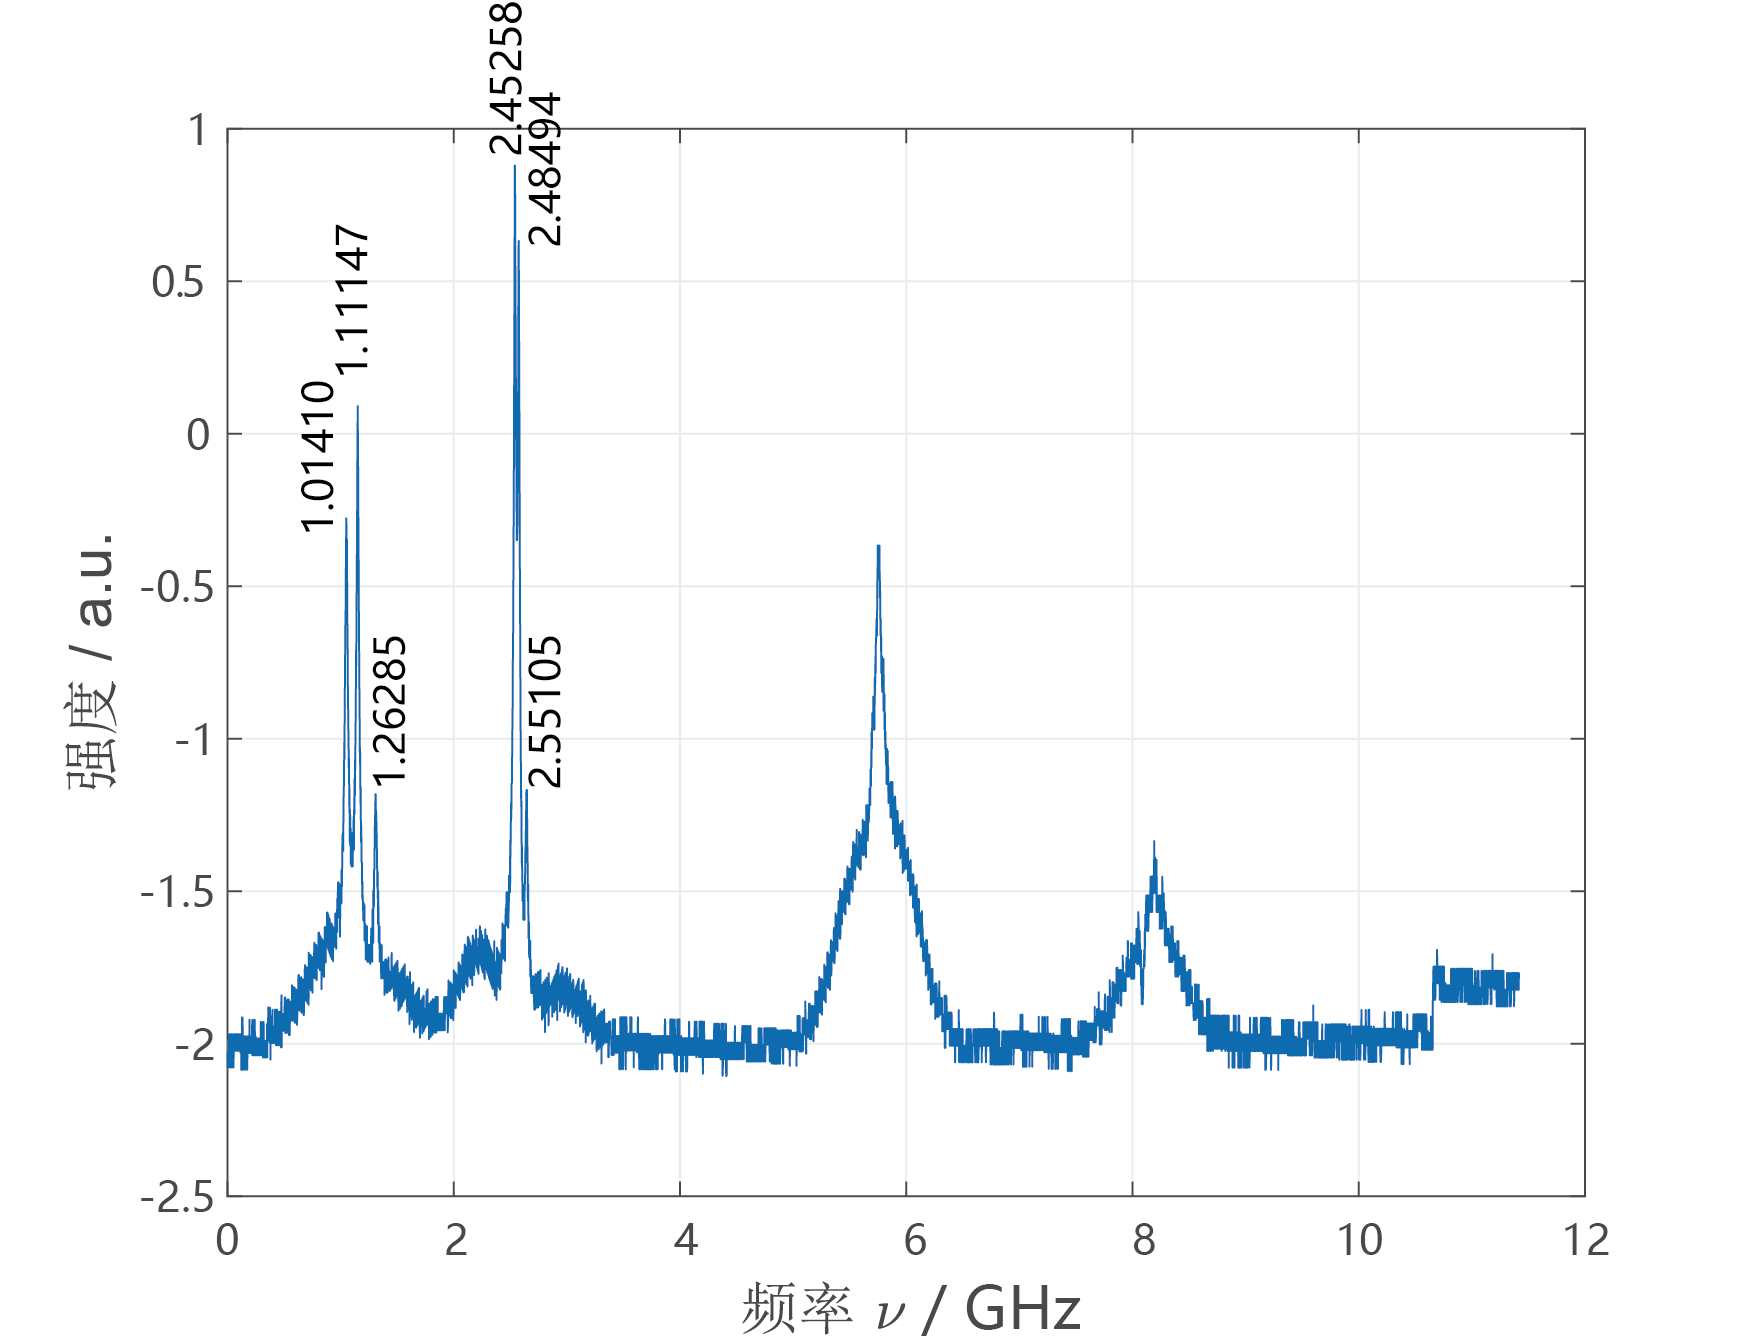
\includegraphics[width=.5\textwidth]{Holeburning-noField.png}
    \caption{无磁场时的烧孔谱线.}
    \label{holeburning-noField}
\end{figure}

如图\ref{B-nu-holeburning}所示,随着磁场的增大,我们还看到了超精细结构的分裂,但是由于数据质量有限,我们并不能准确、定量地将实验中得到的分裂情况与理论对照.

\begin{figure}[ht]
    \centering
    \subfigure[烧孔谱线随磁场变化的情况.]{
    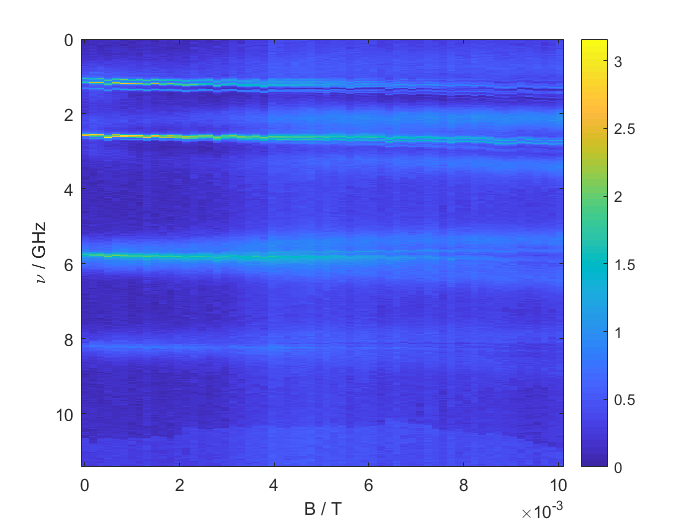
\includegraphics[width=0.45\textwidth]{B-nu-holeburning.png}}
    \subfigure[磁场强度为$0.01$ T时的烧孔谱线.]{
    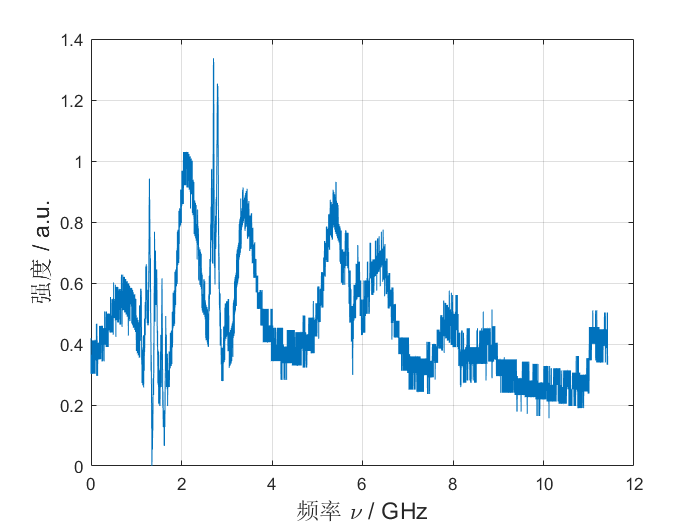
\includegraphics[width=0.45\textwidth]{B-nu-holeburning-strong-field.png}}
    \caption{烧孔谱线随磁场变化的情况.}
    \label{B-nu-holeburning}
\end{figure}

值得一提的是,我们最终没有使用法布里-珀罗腔的透射信号数据来修正示波器时间分辨的误差和激光器频率的漂移,因为我们发现随着磁场的增大,法布里-珀罗腔的透射信号峰向单方向漂移,这一现象的原因尚不明确,可能是因为随着法布里-珀罗腔的温度升高,腔体热胀冷缩导致的共振频率漂移.

\end{document}